% coding:utf-8

%FOSAET, a LaTeX-Code for a electrical summary of basic electronics
%Copyright (C) 2013, Daniel Winz, Ervin Mazlagic

%This program is free software; you can redistribute it and/or
%modify it under the terms of the GNU General Public License
%as published by the Free Software Foundation; either version 2
%of the License, or (at your option) any later version.

%This program is distributed in the hope that it will be useful,
%but WITHOUT ANY WARRANTY; without even the implied warranty of
%MERCHANTABILITY or FITNESS FOR A PARTICULAR PURPOSE.  See the
%GNU General Public License for more details.
%----------------------------------------

\documentclass[a5paper,10pt,fleqn]{book}

\usepackage{layout}

\title{Formelsammlung Elektrotechnik}

\author{Daniel Winz\\Ervin Mazlagi\'c\\Dominik Imhof\\Mario Felder}
\date{\today~\dtc}

\begin{document}

\maketitle
\textbf{}
% coding:utf-8

%FOSAET, a LaTeX-Code for a electrical summary of basic electronics
%Copyright (C) 2013, Daniel Winz, Ervin Mazlagic

%This program is free software; you can redistribute it and/or
%modify it under the terms of the GNU General Public License
%as published by the Free Software Foundation; either version 2
%of the License, or (at your option) any later version.

%This program is distributed in the hope that it will be useful,
%but WITHOUT ANY WARRANTY; without even the implied warranty of
%MERCHANTABILITY or FITNESS FOR A PARTICULAR PURPOSE.  See the
%GNU General Public License for more details.
%----------------------------------------

\chapter*{Über diese Arbeit}
Dies ist das Ergebnis einer Zusammenarbeit auf Basis freier Texte erstellt von Studierenden der Fachhochschule Luzern und ist unter der GPLv2 lizenziert. Der \TeX - bzw. \LaTeX -Code ist auf \url{github.com/fosa/fosaet} hinterlegt.Eine aktuelle PDF-Ausgabe steht auf \url{fosa.adinox.ch} zum Download bereit.

In dieser Formelsammlung sind die Inhalte des ET1-Moduls der HSLU-T\&A zusammengefasst. 

Allfällige Fehler können per E-Mail an die Autoren 
(\href{mailto:info.fosa@gmail.com}{\nolinkurl{info.fosa@gmail.com}}) 
gemeldet werden. 


\tableofcontents

% coding:utf-8

%FOSAET, a LaTeX-Code for a electrical summary of basic electronics
%Copyright (C) 2013, Daniel Winz, Ervin Mazlagic

%This program is free software; you can redistribute it and/or
%modify it under the terms of the GNU General Public License
%as published by the Free Software Foundation; either version 2
%of the License, or (at your option) any later version.

%This program is distributed in the hope that it will be useful,
%but WITHOUT ANY WARRANTY; without even the implied warranty of
%MERCHANTABILITY or FITNESS FOR A PARTICULAR PURPOSE.  See the
%GNU General Public License for more details.
%----------------------------------------

\chapter{Gleichstrom}
\newpage
% coding:utf-8

%FOSAET, a LaTeX-Code for a electrical summary of basic electronics
%Copyright (C) 2013, Daniel Winz, Ervin Mazlagic

%This program is free software; you can redistribute it and/or
%modify it under the terms of the GNU General Public License
%as published by the Free Software Foundation; either version 2
%of the License, or (at your option) any later version.

%This program is distributed in the hope that it will be useful,
%but WITHOUT ANY WARRANTY; without even the implied warranty of
%MERCHANTABILITY or FITNESS FOR A PARTICULAR PURPOSE.  See the
%GNU General Public License for more details.
%----------------------------------------

\section{Zählpfeilsysteme}

\begin{figure}[h!]
	\centering
	\begin{subfigure}[b]{0.4\textwidth}
		\centering
		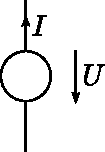
\includegraphics[scale=\schscale]{erzpfeilsys_sch.pdf}
		\caption{Erzeugerpfeilsystem}
		\label{sch:erzpfeilsys}
	\end{subfigure}
	\begin{subfigure}[b]{0.4\textwidth}
		\centering
		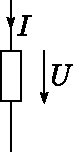
\includegraphics[scale=\schscale]{verbpfeilsys_sch.pdf}
		\caption{Verbraucherpfeilsystem}
		\label{sch:verbpfeilsys}
	\end{subfigure}
	\caption{Zählpfeilsysteme}
	\label{sch:pfeilsys}
\end{figure}

\subsection{Erzeugerpfeilsystem}
Zweipol wirk als Erzeuger, wenn das Produkt aus $U$ und $I$ positiv ist. Sonst wirkt er als Verbraucher. 

\subsection{Verbraucherpfeilsystem}
Zweipol wirk als Verbraucher, wenn das Produkt aus $U$ und $I$ positiv ist. Sonst wirkt er als Erzeuger. 
    % Pfeilsysteme
% coding:utf-8

%FOSAET, a LaTeX-Code for a electrical summary of basic electronics
%Copyright (C) 2013, Daniel Winz, Ervin Mazlagic

%This program is free software; you can redistribute it and/or
%modify it under the terms of the GNU General Public License
%as published by the Free Software Foundation; either version 2
%of the License, or (at your option) any later version.

%This program is distributed in the hope that it will be useful,
%but WITHOUT ANY WARRANTY; without even the implied warranty of
%MERCHANTABILITY or FITNESS FOR A PARTICULAR PURPOSE.  See the
%GNU General Public License for more details.
%----------------------------------------

\section{Ohmsches Gesetz}
\noindent
\[ \begin{array}{l}
U = R \cdot I\\\\
I = \frac{U}{R}\\\\
R = \frac{U}{I}
\end{array}\]
\begin{tabular}{lll}
\multicolumn{2}{l}{Variable}&Einheit\\\\
$U$&Spannung&Volt $[V]$\\\\
$I$&Strom&Ampere $[A]$\\\\
$R$&Widerstand&Ohm $[\Omega]$
\end{tabular}         % Ohmsches Gesetz
% coding:utf-8

%FOSAET, a LaTeX-Code for a electrical summary of basic electronics
%Copyright (C) 2013, Daniel Winz, Ervin Mazlagic

%This program is free software; you can redistribute it and/or
%modify it under the terms of the GNU General Public License
%as published by the Free Software Foundation; either version 2
%of the License, or (at your option) any later version.

%This program is distributed in the hope that it will be useful,
%but WITHOUT ANY WARRANTY; without even the implied warranty of
%MERCHANTABILITY or FITNESS FOR A PARTICULAR PURPOSE.  See the
%GNU General Public License for more details.
%----------------------------------------

\section{Leistung}
\[ P = U \cdot I = \frac{U^2}{R} = I^2 \cdot R \]       % Leistung
% coding:utf-8

%FOSAET, a LaTeX-Code for a electrical summary of basic electronics
%Copyright (C) 2013, Daniel Winz, Ervin Mazlagic

%This program is free software; you can redistribute it and/or
%modify it under the terms of the GNU General Public License
%as published by the Free Software Foundation; either version 2
%of the License, or (at your option) any later version.

%This program is distributed in the hope that it will be useful,
%but WITHOUT ANY WARRANTY; without even the implied warranty of
%MERCHANTABILITY or FITNESS FOR A PARTICULAR PURPOSE.  See the
%GNU General Public License for more details.
%----------------------------------------

\section{Kirchhoffsche Gesetze}

\subsection{Maschenregel}
Die Spannung in einer geschlossenen Masche ist 0. 
\[ \sum U = 0 \]

\subsection{Knotenregel}
Alle Ströme, die in einen Knoten hineinfliessen ergeben in der Summe 0. 
\[ \sum I = 0 \]

\newpage
\subsection{Super-Knoten}
Die Kirchhoff'sche Knotenregel besagt, dass die Summe aller Ströme eines Knoten gleich Null ist.
Dieser Zusammenhang kann auch dann genutzt werden wenn keine idealen Knoten vorhanden sind.
Eine Schaltung kann beliebig zu einen Knoten abstrahiert werden und die Knotenströme zu ermitteln.

\begin{figure}[h!]
\centering
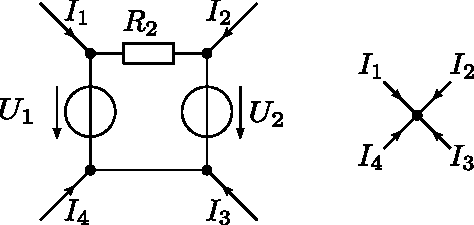
\includegraphics[scale=\schscale]{supernode_sch.pdf}
\caption{Super-Knoten}
\label{sch:supernode}
\end{figure}

\noindent
\textbf{Achtung!} Dieses Prinzip der Zusammenfassung einer Schaltung zu einem Knoten darf nur dazu genutzt werden, um die Ströme in und aus dem Knoten heraus zu ermitteln. Die abstrahierte Schaltung in innern darf jedoch nicht ohne diese Ströme betrachtet werden. 
       % Kirchhoffsche Gesetze


% % coding:utf-8

%FOSAET, a LaTeX-Code for a electrical summary of basic electronics
%Copyright (C) 2013, Daniel Winz, Ervin Mazlagic

%This program is free software; you can redistribute it and/or
%modify it under the terms of the GNU General Public License
%as published by the Free Software Foundation; either version 2
%of the License, or (at your option) any later version.

%This program is distributed in the hope that it will be useful,
%but WITHOUT ANY WARRANTY; without even the implied warranty of
%MERCHANTABILITY or FITNESS FOR A PARTICULAR PURPOSE.  See the
%GNU General Public License for more details.
%----------------------------------------

\chapter{Elektrostatik}
\newpage
%\input{}

% coding:utf-8

%FOSAET, a LaTeX-Code for a electrical summary of basic electronics
%Copyright (C) 2013, Daniel Winz, Ervin Mazlagic

%This program is free software; you can redistribute it and/or
%modify it under the terms of the GNU General Public License
%as published by the Free Software Foundation; either version 2
%of the License, or (at your option) any later version.

%This program is distributed in the hope that it will be useful,
%but WITHOUT ANY WARRANTY; without even the implied warranty of
%MERCHANTABILITY or FITNESS FOR A PARTICULAR PURPOSE.  See the
%GNU General Public License for more details.
%----------------------------------------

\chapter{Wechselstrom}
\newpage
% coding:utf-8

%FOSAET, a LaTeX-Code for a electrical summary of basic electronics
%Copyright (C) 2013, Daniel Winz, Ervin Mazlagic

%This program is free software; you can redistribute it and/or
%modify it under the terms of the GNU General Public License
%as published by the Free Software Foundation; either version 2
%of the License, or (at your option) any later version.

%This program is distributed in the hope that it will be useful,
%but WITHOUT ANY WARRANTY; without even the implied warranty of
%MERCHANTABILITY or FITNESS FOR A PARTICULAR PURPOSE.  See the
%GNU General Public License for more details.
%----------------------------------------

\section{Ausgleichsvorgänge}
\[ y(t) = y_\infty + (y_{0+} - y_\infty) \cdot e^{-\frac{t}{\tau}} \]
       % Ausgleichsvorgänge
% coding:utf-8

%FOSAET, a LaTeX-Code for a electrical summary of basic electronics
%Copyright (C) 2013, Daniel Winz, Ervin Mazlagic

%This program is free software; you can redistribute it and/or
%modify it under the terms of the GNU General Public License
%as published by the Free Software Foundation; either version 2
%of the License, or (at your option) any later version.

%This program is distributed in the hope that it will be useful,
%but WITHOUT ANY WARRANTY; without even the implied warranty of
%MERCHANTABILITY or FITNESS FOR A PARTICULAR PURPOSE.  See the
%GNU General Public License for more details.
%----------------------------------------

\section{Komplexe Impedanz}

\subsubsection{Widerstand}
\[ Z_R = R \]
\[ u_R = R \cdot i_R \]
\begin{figure}[h!]
	\centering
	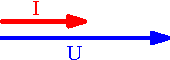
\includegraphics[width=0.3\textwidth]{../fig/zeig_ui_wid.pdf}
	\caption{Zeigerdiagramm Widerstand}
	\label{fig:zeig_ui_wid}
\end{figure}

\newpage
\subsubsection{Kondensator}
\[ Z_C = \frac{1}{j \cdot \omega \cdot C} 
= \frac{1}{j \cdot 2 \cdot \pi \cdot f \cdot C} \]
\[ x_C = Im(Z_C) = -\frac{1}{\omega \cdot C} 
= -\frac{1}{2 \cdot \pi \cdot f \cdot C} \]
\[ u_C = \left( \frac{1}{C} \cdot \int i_C ~ dt \right) + U_C(0) \]
\[ i_C = C \cdot \frac{du_C}{dt} \]
\begin{figure}[h!]
	\centering
	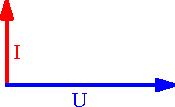
\includegraphics[width=0.3\textwidth]{i../fig/zeig_ui_kap.pdf}
	\caption{Zeigerdiagramm Kondensator}
	\label{fig:zeig_ui_kap}
\end{figure}

\subsubsection{Spule}
\[ Z_L = j \cdot \omega \cdot L = j \cdot 2 \cdot \pi \cdot f \cdot L \]
\[ x_L = Im(Z_L) = \omega \cdot L = 2 \cdot \pi \cdot f \cdot L \]
\[ u_L = L \cdot \frac{di_L}{dt} \]
\[ i_L = \left( \frac{1}{L} \cdot \int u_L ~ dt \right) + I_L(0) \]
\begin{figure}[h!]
	\centering
	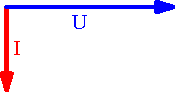
\includegraphics[width=0.3\textwidth]{i../fig/zeig_ui_ind.pdf}
	\caption{Zeigerdiagramm Spule}
	\label{fig:zeig_ui_ind}
\end{figure}
        % Impedanz
% coding:utf-8

%FOSAET, a LaTeX-Code for a electrical summary of basic electronics
%Copyright (C) 2013, Daniel Winz, Ervin Mazlagic

%This program is free software; you can redistribute it and/or
%modify it under the terms of the GNU General Public License
%as published by the Free Software Foundation; either version 2
%of the License, or (at your option) any later version.

%This program is distributed in the hope that it will be useful,
%but WITHOUT ANY WARRANTY; without even the implied warranty of
%MERCHANTABILITY or FITNESS FOR A PARTICULAR PURPOSE.  See the
%GNU General Public License for more details.
%----------------------------------------

\section{Werte von Wechselgrössen}

\subsection{Gleichwert (Mittelwert)}
\[ \overline{U} = \frac{1}{T} \int_0^T u(t) ~ dt \]

\subsection{Gleichrichtwert}
Der Gleichrichtwert bezeichnet den Mittelwert der gleichgereichteten 
Wechselgrösse
\[ \overline{|U|} = \frac{1}{T} \int_0^T |u(t)| ~ dt \]

\subsection{Effektivwert (Quadratischer Mittelwert)}
Der Effektivwert entspricht dem Gleichspannungsewrt, der in einem Widerstand 
die gleiche Leistung umsetzt, wie die Wechselgrösse. 
\[ U_{eff} = \sqrt{\frac{1}{T} \int_0^T u(t)^2 ~ dt} \]

\subsubsection{Effektivwert bei verschiedenen Abschnitten}
\[ U_{eff} = \sqrt{\frac{{U_{eff_1}}^2 \cdot \Delta t_1 
+ {U_{eff_2}}^2 \cdot \Delta t_2 + \dots}{T}} \]

\subsubsection{Mischgrössen}
\[ U_{eff} = \sqrt{{U_{DC}}^2 + {U_{eff_{AC}}}^2} \]

\newpage
\subsubsection{Effektivwert von häufigen Signalformen}
Sinus
\[ U_{eff} = \frac{\hat{u}}{\sqrt{2}} \]
%
Dreieck
\[ U_{eff} = \frac{\hat{u}}{\sqrt{3}} \]
%
Rechteck
\[ U_{eff} = \hat{u} \]
%
Alle Signale müssen symmetrisch sein. 

      % Werte von Wechselgrössen
% coding:utf-8

%FOSAET, a LaTeX-Code for a electrical summary of basic electronics
%Copyright (C) 2013, Daniel Winz, Ervin Mazlagic

%This program is free software; you can redistribute it and/or
%modify it under the terms of the GNU General Public License
%as published by the Free Software Foundation; either version 2
%of the License, or (at your option) any later version.

%This program is distributed in the hope that it will be useful,
%but WITHOUT ANY WARRANTY; without even the implied warranty of
%MERCHANTABILITY or FITNESS FOR A PARTICULAR PURPOSE.  See the
%GNU General Public License for more details.
%----------------------------------------

\section{Leistungsberechnung bei Wechselgrössen}

\subsection{Scheinleistung ($S$)}
\[ S = U_{eff} \cdot I_{eff} \]
\[ S = \sqrt{P^2 + Q^2} \qquad \cos(\varphi) = \frac{P}{S} \]
\[ \underline{S} = P + j Q \]
\[ \underline{S} = S_{eff} \cdot e^{j\varphi} \]
\[ \underline{S} = S_{eff} \angle \varphi \]
\[ \underline{S} = U \cdot I^* = ||I||^2 \cdot \underline{Z} 
= \frac{||U||^2}{\underline{Z}^*} \]

\subsection{Wirkleistung $P$}
\[ P = U_{eff} \cdot I_{eff} \cdot \cos(\varphi) \]

\subsection{Blindleistung $Q$}
\[ Q = U_{eff} \cdot I_{eff} \cdot sin(\varphi) \]

\section{Leistung bei nicht sinusförmigen Grössen}
Momentane Leistung
\[ p(t) = u \cdot i \]
Wirkleistung
\[ P = \frac{1}{T} \int_{0}^{T} p(t) dt 
= \frac{1}{T} \int_{0}^{T} u \cdot i ~ dt \]
Wirkleistung mit Fourierreihe
\[ P = \sum_{v=0}^{\infty} \frac{\hat{u}_v 
\cdot \hat{i}_v}{2} \cdot \cos(\varphi_v) \]
\[ \varphi_v = \varphi_{u_v} - \varphi_{i_v} 
\qquad \text{mit gleichen Frequenzen von $u$ und $i$} \]
Scheinleistung
\[ S = U \cdot I \]
Leistungsfaktor
\[ \lambda = \frac{P}{S} \]
Blindleistung
\[ Q^2 = S^2 - P^2 \]
Spezialfall: $u = \hat{U} \cdot \sin(\omega_1 \cdot t) ~ \text{und} ~ i 
= I_{AV} + \sum\limits_{v=1}^{\infty} \hat{I}_v \cdot 
\sin(v\cdot \omega_1 \cdot t + \varphi_v)$
\[ \begin{array}{@{}ll}
P = U \cdot I \cdot \cos(\varphi_1) \\
\varphi_1 = \varphi_u - \varphi_{i_1} \\
Q_1 = U \cdot I_1 \cdot \sin(\varphi_1) &\text{Grundschwingungsblindleistung} \\
S_1 = U \cdot I_1 &\text{Grundschwingungsscheinleistung} \\
S^2 = P^2 + {Q_1}^2 + D^2 \\
D = {Q_2} + {Q_3} + \dots + {Q_\infty} & \text{Verzerrungsblindleistung} \\
\end{array}  \]     % Leistungsberechnung bei Wechselgrössen

% coding:utf-8

%FOSAET, a LaTeX-Code for a electrical summary of basic electronics
%Copyright (C) 2013, Daniel Winz, Ervin Mazlagic

%This program is free software; you can redistribute it and/or
%modify it under the terms of the GNU General Public License
%as published by the Free Software Foundation; either version 2
%of the License, or (at your option) any later version.

%This program is distributed in the hope that it will be useful,
%but WITHOUT ANY WARRANTY; without even the implied warranty of
%MERCHANTABILITY or FITNESS FOR A PARTICULAR PURPOSE.  See the
%GNU General Public License for more details.
%----------------------------------------

\chapter{Drehstrom}
\newpage
%\input{}
%
$U$: Aussenleiterspannung

$U_s$: Strangspannung
\[ U_s = \frac{U}{\sqrt{3}} \]
\[ \begin{array}{@{}l@{}l@{}l@{}r}
U_{1N} &= U_s &\angle &   0^\circ \\
U_{2N} &= U_s &\angle &-120^\circ \\
U_{3N} &= U_s &\angle & 120^\circ \\
U_{12} &= U   &\angle &  30^\circ \\
U_{23} &= U   &\angle & -90^\circ \\
U_{31} &= U   &\angle & 150^\circ 
\end{array} \]
\[ Y_1 = \frac{1}{Z_1} \]
\[ Y_2 = \frac{1}{Z_2} \]
\[ Y_3 = \frac{1}{Z_3} \]
\[ Y_n = \frac{1}{Z_n} \]
\[ U_{KN} = \frac{Y_1 \cdot U_{1N} + Y_2 \cdot U_{2N} + Y_3 \cdot U_{3N}}
{Y_1 + Y_2 + Y_3 + Y_N} \]
\begin{figure}[h!]
  \centering
  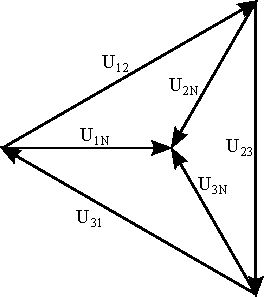
\includegraphics[width=0.3\textwidth]{drehstrom.pdf}
  \caption{Zeigerdiagramm Drehstrom}
  \label{fig:zeig_dreh}
\end{figure}


% coding:utf-8

%FOSAET, a LaTeX-Code for a electrical summary of basic electronics
%Copyright (C) 2013, Daniel Winz, Ervin Mazlagic

%This program is free software; you can redistribute it and/or
%modify it under the terms of the GNU General Public License
%as published by the Free Software Foundation; either version 2
%of the License, or (at your option) any later version.

%This program is distributed in the hope that it will be useful,
%but WITHOUT ANY WARRANTY; without even the implied warranty of
%MERCHANTABILITY or FITNESS FOR A PARTICULAR PURPOSE.  See the
%GNU General Public License for more details.
%----------------------------------------

\chapter{Schaltungstechnik}
\newpage
% coding:utf-8

%FOSAET, a LaTeX-Code for a electrical summary of basic electronics
%Copyright (C) 2013, Daniel Winz, Ervin Mazlagic

%This program is free software; you can redistribute it and/or
%modify it under the terms of the GNU General Public License
%as published by the Free Software Foundation; either version 2
%of the License, or (at your option) any later version.

%This program is distributed in the hope that it will be useful,
%but WITHOUT ANY WARRANTY; without even the implied warranty of
%MERCHANTABILITY or FITNESS FOR A PARTICULAR PURPOSE.  See the
%GNU General Public License for more details.
%----------------------------------------

\section{Spannungsteiler}

\subsection{unbelasteter Spannungsteiler}
\begin{figure}[h!]
	\centering
	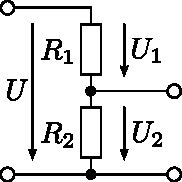
\includegraphics[scale=\schscale]{uteil.pdf}
	\caption{unbelasteter Spannungsteiler}
	\label{sch:uteil}
\end{figure}
\[ U_2 = \frac{U_1}{R_1 + R_2} \cdot R_2 \]

\subsection{belasteter Spannungsteiler}
\begin{figure}[h!]
	\centering
	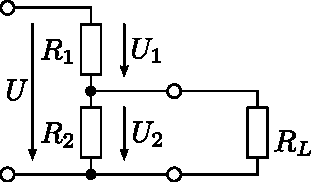
\includegraphics[scale=\schscale]{uteilbel.pdf}
	\caption{belasteter Spannungsteiler}
	\label{sch:uteilbel}
\end{figure}
\[ U_2 = \frac{U_1}{R_1 + \frac{R_2 \cdot R_L}{R_2 + R_L}} \cdot \frac{R_2 \cdot R_L}{R_2 + R_L} \]

\newpage
\subsection{unbelastetes Potentiometer}
\begin{figure}[h!]
	\centering
	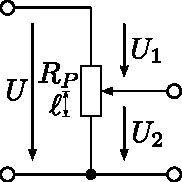
\includegraphics[scale=\schscale]{poti.pdf}
	\caption{unbelastetes Potentiometer}
	\label{sch:poti}
\end{figure}
\[ U_2 = U_1 \cdot \ell \]

\subsection{belastetes Potentiometer}
\begin{figure}[h!]
	\centering
	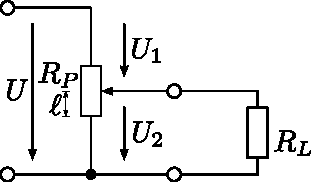
\includegraphics[scale=\schscale]{potibel.pdf}
	\caption{belastetes Potentiometer}
	\label{sch:potibel}
\end{figure}
\[ U_2 = \frac{U_1}{R_p \cdot (1 - \ell) + \frac{R_p \cdot \ell \cdot R_L}{R_p \cdot \ell + R_L}} \cdot \frac{R_p \cdot \ell \cdot R_L}{R_p \cdot \ell + R_L} \]
       % Spannungsteiler
% coding:utf-8

%FOSAET, a LaTeX-Code for a electrical summary of basic electronics
%Copyright (C) 2013, Daniel Winz, Ervin Mazlagic

%This program is free software; you can redistribute it and/or
%modify it under the terms of the GNU General Public License
%as published by the Free Software Foundation; either version 2
%of the License, or (at your option) any later version.

%This program is distributed in the hope that it will be useful,
%but WITHOUT ANY WARRANTY; without even the implied warranty of
%MERCHANTABILITY or FITNESS FOR A PARTICULAR PURPOSE.  See the
%GNU General Public License for more details.
%----------------------------------------

\section{Stromteiler}
\begin{figure}[h!]
	\centering
	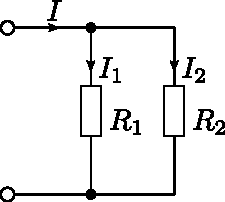
\includegraphics[scale=\schscale]{iteil.pdf}
	\caption{Stromteiler}
	\label{sch:iteil}
\end{figure}
\[ I_2 = I \cdot \frac{R_1}{R_1 + R_2} \]

\subsubsection{Stromteiler mit $> 2$ Widerständen}
\[ I_n = I_q \cdot \frac{(R1 // R2 \dots // R_{n-1})}
{(R1 // R2 \dots // R_{n-1}) + R_n} 
= I_q \cdot \frac{\left(\frac{R_1 \cdot R_2 \dots R_{n-1}}
{R_1 + R_2 \dots R_{n-1}}\right)}
{\left(\frac{R_1 \cdot R_2 \dots R_{n-1}}
{R_1 + R_2 \dots R_{n-1}}\right) + R_n} \]       % Stromteiler
% coding:utf-8

%FOSAET, a LaTeX-Code for a electrical summary of basic electronics
%Copyright (C) 2013, Daniel Winz, Ervin Mazlagic

%This program is free software; you can redistribute it and/or
%modify it under the terms of the GNU General Public License
%as published by the Free Software Foundation; either version 2
%of the License, or (at your option) any later version.

%This program is distributed in the hope that it will be useful,
%but WITHOUT ANY WARRANTY; without even the implied warranty of
%MERCHANTABILITY or FITNESS FOR A PARTICULAR PURPOSE.  See the
%GNU General Public License for more details.
%----------------------------------------

\newpage
\section{Brückenschaltung}
\begin{figure}[h!]
  \centering
  \begin{circuitikz}[scale=1]\draw
    (1.5,6) to[short, o-*] (1.5,5)
    (1.5,1) to[short, *-o] (1.5,0)
    (0,5) to[short, ] (3,5)
    (0,1) to[short, ] (3,1)
    (0,5) to[R=$R_1$, ] (0,3)
    (0,3) to[R=$R_2$, ] (0,1)
    (3,5) to[R=$R_3$, ] (3,3)
    (3,3) to[R=$R_4$, ] (3,1)
    (0,3) to[R=$R_5$, *-*] (3,3)
    ;
  \end{circuitikz}
  \caption{Brückenschaltung}
\end{figure}

\subsubsection{Abgeglichene Brückenschaltung}
\[ \frac{R_1}{R_2} = \frac{R_3}{R_4} \]
\[ U_5 = U_2 - U_4 = 0 \]
\[ I_5 = 0 \]

\subsubsection{Nicht abgegelichen ohne $R_5$}
\[ U_5 = U_2 - U_4 = U_q \cdot \left( \left( \frac{R_2}{R_1 + R_2} \right) - 
\left( \frac{R_4}{R_3 + R_4} \right) \right) \]

\subsubsection{Nicht abgeglichen}
\begin{scriptsize}
\[ U_5 = U_q \cdot \frac{(R_2 \cdot R_3 - R_1 \cdot R_4) \cdot R_5}
{R_5 \cdot (R_3 + R_4) \cdot (R_1 + R_2) 
+ R_1 \cdot R_3 \cdot R_4 + R_2 \cdot R_3 \cdot R_4 
+ R_1 \cdot R_2 \cdot R_3 + R_1 \cdot R_2 \cdot R_4} \]
\[ I_5 = U_q \cdot \frac{R_2 \cdot R_3 - R_1 \cdot R_4}
{R_5 \cdot (R_3 + R_4) \cdot (R_1 + R_2) 
+ R_3 \cdot R_4 \cdot (R_1 + R_2) + R_1 \cdot R_2 \cdot (R_3 + R_4)} \]
\end{scriptsize}      % Brückenschaltung
% coding:utf-8

%FOSAET, a LaTeX-Code for a electrical summary of basic electronics
%Copyright (C) 2013, Daniel Winz, Ervin Mazlagic

%This program is free software; you can redistribute it and/or
%modify it under the terms of the GNU General Public License
%as published by the Free Software Foundation; either version 2
%of the License, or (at your option) any later version.

%This program is distributed in the hope that it will be useful,
%but WITHOUT ANY WARRANTY; without even the implied warranty of
%MERCHANTABILITY or FITNESS FOR A PARTICULAR PURPOSE.  See the
%GNU General Public License for more details.
%----------------------------------------

\section{Leistungsanpassung}
Soll einer Quelle die maximal mögliche Leistung entnommen werden, so wird 
Leistungsanpassung vorgenommen. Bei Leistungsanpassung entspricht der Wert des 
Lastwiderstandes demjenigen des Innenwiderstandes der Quelle. 
\[ R_L = R_i \]
\[ P = \frac{\frac{U_q}{2}}{R_l} \]

\subsubsection{Leistungsanpassung bei komplexen Impedanzen}
$R_L$ Real: 
\[ R_L = ||Z_i|| \]
$Z_L$ Komplex: 
\[ Z_L = {Z_i}^* \]      % Leistungsanpassung
% coding:utf-8

%FOSAET, a LaTeX-Code for a electrical summary of basic electronics
%Copyright (C) 2013, Daniel Winz, Ervin Mazlagic

%This program is free software; you can redistribute it and/or
%modify it under the terms of the GNU General Public License
%as published by the Free Software Foundation; either version 2
%of the License, or (at your option) any later version.

%This program is distributed in the hope that it will be useful,
%but WITHOUT ANY WARRANTY; without even the implied warranty of
%MERCHANTABILITY or FITNESS FOR A PARTICULAR PURPOSE.  See the
%GNU General Public License for more details.
%----------------------------------------

\newpage
\section{Umwandlung Spannungsquelle $\leftrightarrow$ Stromquelle}

\subsection{Thévenin-Theorem}
Nach Thévenin kann jedes Netzwerk bestehend aus Strom-, Spannungsquellen und Widerständen in eine Ersatzspannungsquelle\footnote{Thévenin-Äquivalent} gewandelt werden.

\begin{figure}[h!]
\centering
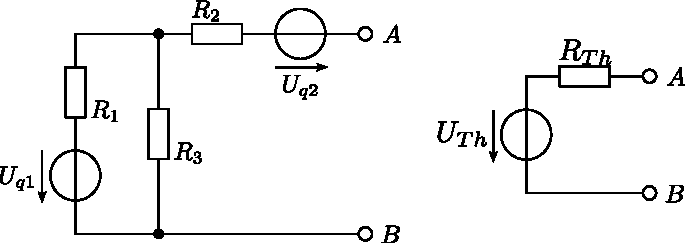
\includegraphics[scale=\schscale]{thevenin_sch_2.pdf}
\caption{Schaltung (l) und ihr Thévenin-Äquivalent (r)}
\label{sch:thevenin}
\end{figure}

\subsubsection{Berechnung}
\begin{itemize}
\item Leerlaufspannung $U_{Th}$ bestimmen (siehe Kapitel~\ref{sec:superpos})
\item Ersatzwiderstand ermitteln durch ausschalten aller unabhängiger Quellen (Spannungsquellen werden kurzgeschlossen, Stromquellen unterbrochen)
\end{itemize}

\newpage
\subsection{Norton-Theorem}
Nach Norton kann jedes Netzwerk bestehend aus Strom-, Spannungsquellen und Widerständen in eine Ersatzstromquelle\footnote{Norton-Äqivalent} gewandelt werden.

\begin{figure}[h!]
\centering
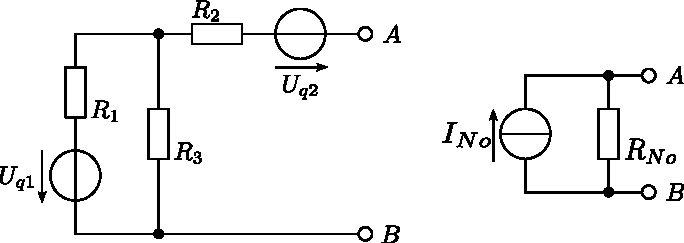
\includegraphics[scale=\schscale]{norton_sch_2.pdf}
\caption{Schaltung (l) und ihr Norton-Äquivalent (r)}
\label{sch:norton}
\end{figure}

\subsection{Spannungsquelle $\rightarrow$ Stromquelle}
\[ R_{No} = R_{Th} \]
\[ I_q = \frac{U_q}{R_{Th}} \]

\subsection{Stromquelle $\rightarrow$ Spannungsquelle}
\[ R_{Th} = R_{No} \]
\[ U_q = I_q \cdot R_{No} \]
    % Umwandlung Spannungsquelle <-> Stromquelle
% coding:utf-8

%FOSAET, a LaTeX-Code for a electrical summary of basic electronics
%Copyright (C) 2013, Daniel Winz, Ervin Mazlagic

%This program is free software; you can redistribute it and/or
%modify it under the terms of the GNU General Public License
%as published by the Free Software Foundation; either version 2
%of the License, or (at your option) any later version.

%This program is distributed in the hope that it will be useful,
%but WITHOUT ANY WARRANTY; without even the implied warranty of
%MERCHANTABILITY or FITNESS FOR A PARTICULAR PURPOSE.  See the
%GNU General Public License for more details.
%----------------------------------------

\section{Umwandlung Stern $\leftrightarrow$ Dreieck}
\begin{figure}[h!]
	\centering
	\begin{subfigure}[b]{0.4\textwidth}
		\centering
		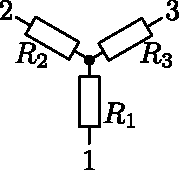
\includegraphics[scale=\schscale]{star_sch.pdf}
		\caption{Sternschaltung}
		\label{sch:star}
	\end{subfigure}
	\begin{subfigure}[b]{0.4\textwidth}
		\centering
		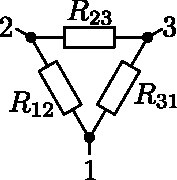
\includegraphics[scale=\schscale]{tri_sch.pdf}
		\caption{Dreieckschaltung}
		\label{sch:tri}
	\end{subfigure}
	\caption{Stern und Dreieckschaltung}
	\label{sch:tristar}
\end{figure}


\subsection{Umwandlung Dreieck $\to$ Stern}
\[ \begin{matrix}
R_1 = \dfrac{R_{12} \cdot R_{31}}{R_{12} + R_{23} + R_{31}}\\\\
R_2 = \dfrac{R_{23} \cdot R_{12}}{R_{12} + R_{23} + R_{31}}\\\\
R_3 = \dfrac{R_{31} \cdot R_{23}}{R_{12} + R_{23} + R_{31}}\\\\
\end{matrix} \]

\subsection{Umwandlung Stern $\to$ Dreieck}
\[ \begin{matrix}
R_{12} = \dfrac{R_1 \cdot R_2 + R_2 \cdot R_3 + R_3 \cdot R_1}{R_3}\\\\
R_{23} = \dfrac{R_1 \cdot R_2 + R_2 \cdot R_3 + R_3 \cdot R_1}{R_1}\\\\
R_{31} = \dfrac{R_1 \cdot R_2 + R_2 \cdot R_3 + R_3 \cdot R_1}{R_2}\\\\
\end{matrix} \]

\subsection{Umwandlung Dreieck $\to$ Stern mit identischen Widerständen}
\[ R_{\upY} = \frac{R_{\triangle}}{3} \]

\subsection{Umwandlung Stern $\to$ Dreieck mit identischen Widerständen}
\[ R_{\triangle} = 3 \cdot R_{\upY} \]     % Dreieck <-> Stern Umwandlung
% coding:utf-8

%FOSAET, a LaTeX-Code for a electrical summary of basic electronics
%Copyright (C) 2013, Daniel Winz, Ervin Mazlagic

%This program is free software; you can redistribute it and/or
%modify it under the terms of the GNU General Public License
%as published by the Free Software Foundation; either version 2
%of the License, or (at your option) any later version.

%This program is distributed in the hope that it will be useful,
%but WITHOUT ANY WARRANTY; without even the implied warranty of
%MERCHANTABILITY or FITNESS FOR A PARTICULAR PURPOSE.  See the
%GNU General Public License for more details.
%----------------------------------------

\section{Quellenvereinfachung}
Interessiert die Leistung an der Quelle nicht oder ist die Spannung an 
Stromquellen oder der Strom durch Spannungsquellen nicht wichtig, können 
Quellen wie folgt vereinfacht werden. 
\begin{center}
\begin{minipage}[c]{0.3\textwidth}
\begin{circuitikz}[scale=1]\draw
  (0,5) to[V=$U_q$, o-] (0,3)
  (0,3) to[I=$I_q$, -o] (0,1)
  ;
\end{circuitikz}
\end{minipage}
\begin{minipage}[c]{0.1\textwidth}
\Huge$\Rightarrow$
\end{minipage}
\begin{minipage}[c]{0.3\textwidth}
\begin{circuitikz}[scale=1]\draw
  (2,4) to[I=$I_q$, o-o] (2,2)
  ;
\end{circuitikz}
\end{minipage}
\end{center}
%
\begin{center}
\begin{minipage}[c]{0.3\textwidth}
\begin{circuitikz}[scale=1]\draw
  (1,4) to[short, o-*] (1,3)
  (0,3) to[short, ] (2,3)
  (0,1) to[short, ] (2,1)
  (1,1) to[short, *-o] (1,0)
  (0,3) to[V=$U_q$, ] (0,1)
  (2,3) to[I=$I_q$, ] (2,1)
  ;
\end{circuitikz}
\end{minipage}
\begin{minipage}[c]{0.1\textwidth}
\Huge$\Rightarrow$
\end{minipage}
\begin{minipage}[c]{0.3\textwidth}
\begin{circuitikz}[scale=1]\draw
  (4,3) to[V=$U_q$, o-o] (4,1)
  ;
\end{circuitikz}
\end{minipage}
\end{center}
%
\begin{center}
\begin{minipage}[c]{0.3\textwidth}
\begin{circuitikz}[scale=1]\draw
  (0,5) to[R=$R$, o-] (0,3)
  (0,3) to[I=$I_q$, -o] (0,1)
  ;
\end{circuitikz}
\end{minipage}
\begin{minipage}[c]{0.1\textwidth}
\Huge$\Rightarrow$
\end{minipage}
\begin{minipage}[c]{0.3\textwidth}
\begin{circuitikz}[scale=1]\draw
  (2,4) to[I=$I_q$, o-o] (2,2)
  ;
\end{circuitikz}
\end{minipage}
\end{center}
%
\begin{center}
\begin{minipage}[c]{0.3\textwidth}
\begin{circuitikz}[scale=1]\draw
  (1,4) to[short, o-*] (1,3)
  (0,3) to[short, ] (2,3)
  (0,1) to[short, ] (2,1)
  (1,1) to[short, *-o] (1,0)
  (0,3) to[V=$U_q$, ] (0,1)
  (2,3) to[R=$R$, ] (2,1)
  ;
\end{circuitikz}
\end{minipage}
\begin{minipage}[c]{0.1\textwidth}
\Huge$\Rightarrow$
\end{minipage}
\begin{minipage}[c]{0.3\textwidth}
\begin{circuitikz}[scale=1]\draw
  (4,3) to[V=$U_q$, o-o] (4,1)
  ;
\end{circuitikz}
\end{minipage}
\end{center}
%
       % Quellenvereinfachung
% coding:utf-8

%FOSAET, a LaTeX-Code for a electrical summary of basic electronics
%Copyright (C) 2013, Daniel Winz, Ervin Mazlagic

%This program is free software; you can redistribute it and/or
%modify it under the terms of the GNU General Public License
%as published by the Free Software Foundation; either version 2
%of the License, or (at your option) any later version.

%This program is distributed in the hope that it will be useful,
%but WITHOUT ANY WARRANTY; without even the implied warranty of
%MERCHANTABILITY or FITNESS FOR A PARTICULAR PURPOSE.  See the
%GNU General Public License for more details.
%----------------------------------------

\newpage
\section{Quellenverschiebung}
Das Verschieben von Quellen kann notwendig sein, wenn zum Beispiel beim Knotenpotentialverfahren eine ideale Spannungsquelle nicht in eine Stromquelle umgewandelt werden kann. 

\subsection{Verschiebung von Spannungsquellen}
\begin{enumerate}
  \item Knoten bestimmen, über welchen die Spannungsquelle verschoben werden soll. 
  \item Spannungsquelle vervielfachen und über Knoten verschieben. \\
  Dabei muss die Spannungsquelle auf jede Leitung verschoben werden, welche zum Knoten führt. Somit werden die Maschengleichungen nicht verändert. 
\end{enumerate}
% Spannungsquellen können über einen Knoten hinweg geschoben werden. Bei der Verschiebung muss er vervielfacht werden und auf jede andere Leitung am Knoten eingefügt werden. 
\begin{figure}[h!]
	\centering
	\begin{subfigure}[b]{0.4\textwidth}
		\centering
		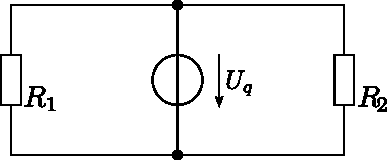
\includegraphics[scale=\schscalesmall]{../fig/qversch_uq1_sch.pdf}
% 		\caption{1}
		\label{sch:starqversch_uq1}
	\end{subfigure}
	\begin{subfigure}[b]{0.4\textwidth}
		\centering
		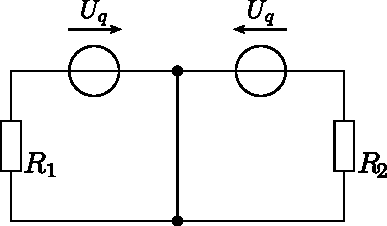
\includegraphics[scale=\schscalesmall]{../fig/qversch_uq2_sch.pdf}
% 		\caption{2}
		\label{sch:qversch_uq2}
	\end{subfigure}
	\caption{Verschiebung von Spannungsquellen}
	\label{sch:qversch_uq1}
\end{figure}

\newpage
\subsection{Verschiebung von Stromquellen}
\begin{enumerate}
  \item Masche bestimmen, innerhalb welcher die Stromquelle verschoben werden soll. 
  \item Stromquelle vervielfachen. 
  \item Stromquellen verschieben, dass zwischen jedem Knoten ausser an der Stelle der vorherigen Stromquelle eine Stromquelle zu liegen kommt. 
\end{enumerate}
% Stromquellen werden zunächst vervielfacht und anschliessend innerhalb der Masche an jeden Knoten "umgehängt". 
\begin{figure}[h!]
	\centering
	\begin{subfigure}[b]{0.3\textwidth}
		\centering
		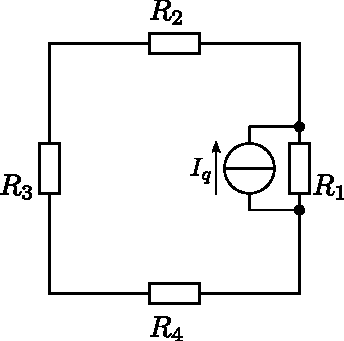
\includegraphics[scale=\schscalesmall]{../fig/qversch_iq1_sch.pdf}
% 		\caption{1}
		\label{sch:qversch_iq1}
	\end{subfigure}
	\begin{subfigure}[b]{0.3\textwidth}
		\centering
		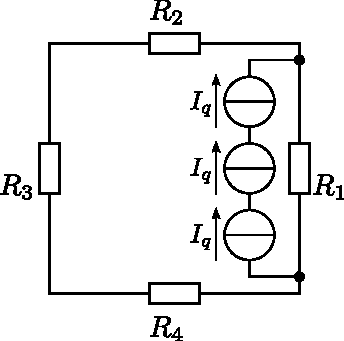
\includegraphics[scale=\schscalesmall]{../fig/qversch_iq2_sch.pdf}
% 		\caption{2}
		\label{sch:qversch_iq2}
	\end{subfigure}
	\begin{subfigure}[b]{0.3\textwidth}
		\centering
		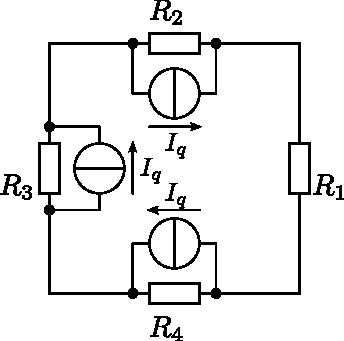
\includegraphics[scale=\schscalesmall]{../fig/qversch_iq3_sch.pdf}
% 		\caption{3}
		\label{sch:qversch_iq3}
	\end{subfigure}
	\caption{Verschiebung von Stromquellen}
	\label{sch:qversch_iq}
\end{figure}
     % Quellenverschiebung
% coding:utf-8

%FOSAET, a LaTeX-Code for a electrical summary of basic electronics
%Copyright (C) 2013, Daniel Winz, Ervin Mazlagic

%This program is free software; you can redistribute it and/or
%modify it under the terms of the GNU General Public License
%as published by the Free Software Foundation; either version 2
%of the License, or (at your option) any later version.

%This program is distributed in the hope that it will be useful,
%but WITHOUT ANY WARRANTY; without even the implied warranty of
%MERCHANTABILITY or FITNESS FOR A PARTICULAR PURPOSE.  See the
%GNU General Public License for more details.
%----------------------------------------

\section{Superposition}
\label{sec:superpos}
Unter Superposition bzw. Überlagerung versteht man, dass gleiche Grössen sich linear überlagern.
In der Elektrotechnik z.B. bei der bestimmung von Netzwerkspannungen. 
So kann ein Netzwerk mit mehreren Quellen per Superposition einfach analysiert werden, indem man das Netzwerk mit jeweils einer aktiver Quelle betrachtet. 
Unabhängige Spannungsquellen werden kurzgeschlossen und unabhängige Stromquellen unterbrochen.
Die Ergenisse jeder Betrachtung können dann linear kombiniert bzw. überlagert werden.
    % Superposition bzw. Überlagerung
% coding:utf-8

%FOSAET, a LaTeX-Code for a electrical summary of basic electronics
%Copyright (C) 2013, Daniel Winz, Ervin Mazlagic

%This program is free software; you can redistribute it and/or
%modify it under the terms of the GNU General Public License
%as published by the Free Software Foundation; either version 2
%of the License, or (at your option) any later version.

%This program is distributed in the hope that it will be useful,
%but WITHOUT ANY WARRANTY; without even the implied warranty of
%MERCHANTABILITY or FITNESS FOR A PARTICULAR PURPOSE.  See the
%GNU General Public License for more details.
%----------------------------------------

\newpage
\section{Knotenpotentialverfahren}
\begin{enumerate}
  \item Alle realen Spannungsquellen in Stromquellen umwandeln. 
  \item Null-Potential ($N_0$) wählen (bestenfalls dort wo der Strom gesucht ist)
  \item restliche Knoten nummerieren ($N_1$, $N_2$, $N_3$ ...$N_n$)
  \item Matrix aufstellen
  \item Links alle Knoten ohne den Bezugsknoten auflisten
  \item Oben alle Spannungen von den Knoten zum Bezugsknoten eintragen
  \item Hauptdiagonale ausfüllen: \\
  Dazu sind die Leitwerte aller Widerstände, die am jeweiligen Knoten angeschlossen sind zu addieren und hinzuschreiben. 
  \item Restliche Matrix ausfüllen: \\
  Dazu sind die Leitwerte aller Widerstände, die direkt zwischen den jeweiligen Knoten liegen zu addieren und einzutragen. Das Vorzeichen ist dabei immer negativ. Die Hauptachse bildet dabei eine Symmetrieachse. \\
  Liegt keine direkte Verbindung zwischen zwei Knoten, so wird 0 eingetragen
  \item In der rechten Spalte Stromquellen eintragen. \\
  Das Vorzeichen ist dabei abhängig von der Flussrichtung: \\
  \begin{itemize}
    \item[+] wenn der Strom in den Knoten fliesst
    \item[-] wenn der Strom vom Knoten weg fliesst
  \end{itemize}
\end{enumerate}

\newpage
\subsection{Beispiel}

\begin{figure}[h!]
\centering
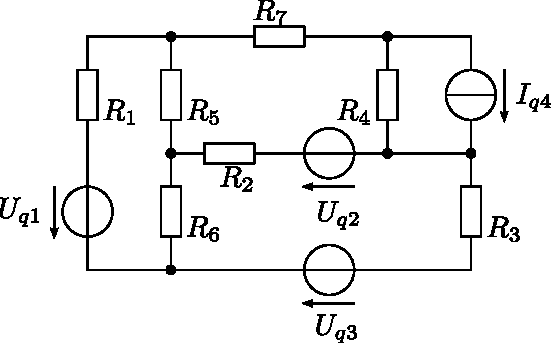
\includegraphics[scale=\schscale]{knotpot_sch.pdf}
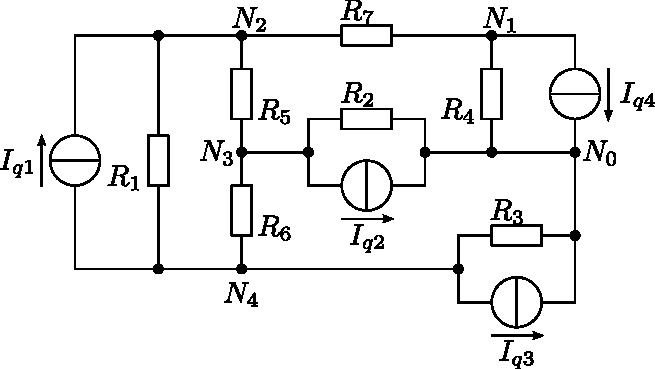
\includegraphics[scale=\schscale]{knotpot_sch_2.pdf}
\caption{Umwandlung von Strom- zu Spannungsquellen}
\label{sch:knotpot_2}
\end{figure}

\begin{table}[h!]
\footnotesize
\[ 	\begin{array}{c|cccc||c}
	N & U_{10}						& U_{20}										& U_{30} 											& U_{40} 											& I \\
	\hline &&&&& \\
	N_1	& \frac{1}{R_4} + \frac{1}{R_7}		& -\frac{1}{R_7} 								& 0 												& 0 												& -I_{q4} 			\\
	&&&&& \\
	N_2	& -\frac{1}{R_7} 					& \frac{1}{R_1} + \frac{1}{R_5} + \frac{1}{R7} 	& -\frac{1}{R_5} 									& -\frac{1}{R_1} 									& I_{q1} 			\\ 
	&&&&& \\
	N_3	& 0 								& -\frac{1}{R_5} 								& \frac{1}{R_2} + \frac{1}{R_5} + \frac{1}{R_6} 	& -\frac{1}{R_6} 									& -I_{q2} 			\\ 
	&&&&& \\
	N_4 & 0 								& -\frac{1}{R_1} 								& -\frac{1}{R_6} 									& \frac{1}{R_1} + \frac{1}{R_3} + \frac{1}{R_6} 	& -I_{q2} -I_{q3} 	\\ 
	&&&&& \\
	\end{array}
\]
\normalsize
\caption{Matrix zu Abb.~\ref{sch:knotpot_2}}
\end{table}

\newpage
     % Knotenpotentialverfahren
% coding:utf-8

%FOSAET, a LaTeX-Code for a electrical summary of basic electronics
%Copyright (C) 2013, Daniel Winz, Ervin Mazlagic

%This program is free software; you can redistribute it and/or
%modify it under the terms of the GNU General Public License
%as published by the Free Software Foundation; either version 2
%of the License, or (at your option) any later version.

%This program is distributed in the hope that it will be useful,
%but WITHOUT ANY WARRANTY; without even the implied warranty of
%MERCHANTABILITY or FITNESS FOR A PARTICULAR PURPOSE.  See the
%GNU General Public License for more details.
%----------------------------------------

\section{Maschenstromverfahren}

\begin{itemize}
	\item Alle realen Quellen in Spannungsquellen wandeln
	\item Maschen legen und nummerieren ($M_1$, $M_2$, $M_3$ ...$M_n$)
	\item Baum bilden (Baum bedeutet hier ein Strang, welcher alle Knoten berührt und durchgehend verbunden ist. Dieser muss keine \textit{Schlange} darstellen, sondern darf auch sternförmig etc. sein.
	\item Matrix aufstellen
	\item Links alle Maschen auflisten
	\item Oben alle Ströme der Quellen eintragen welche zwischen Knoten liegen (nicht jener die innerhalb des Baumes liegen)
	\item Hauptdiagonale ausfüllen:\\ Hierzu sind alle Widerstandswerte zu summieren welche in entsprechender Masche liegen.
	\item Restliche Matrix ausfüllen:\\ Hierzu sind alle Widerstandswerte einzutragen welche zu zwei Maschen gehören einzutragen. Das Vorzeichen ist positiv zu wählen, falls die Maschenpfeilrichtung die selbe ist, sonst negativ.
	\item In der rechten Spalte Spannungsquellen eintragen. Das Vorzeichen ist dabei positiv, falls die Maschenpfeilrichtung entgegen der Spannungspfeilrichtung ist, sonst negativ.
\end{itemize}

\newpage

\subsection{Beispiel}
\begin{figure}[h!]
\centering
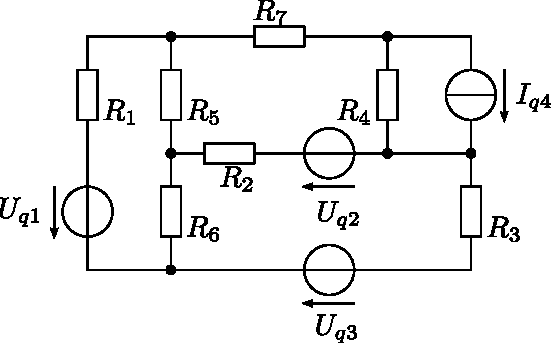
\includegraphics[scale=\schscale]{../fig/mastro_sch.pdf}

\vspace{5mm}

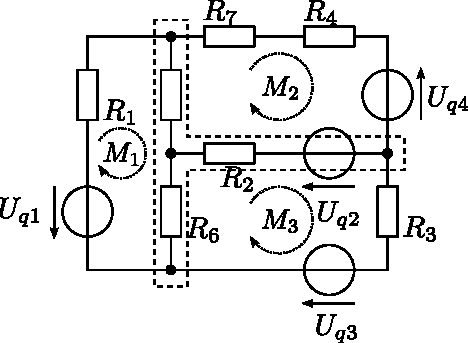
\includegraphics[scale=\schscale]{../fig/mastro_sch_2.pdf}
\caption{Schaltung zum Maschenstromverfahren}
\label{sch:mastro}
\end{figure}

\begin{table}[h!]
\footnotesize
\[ \begin{array}{c|ccc||c}

M	& I_1 & I_2 & I_3 & U \\
\hline &&&& \\
M_1 	& R_1 + R_5 + R_6 	& -R_5 				& -R_6 			& U_{q1} \\
&&&& \\
M_2 	& -R_5 			& R_2 + R_4 + R_5 + R_7 	& -R_2 			& U_{q4} \\
&&&& \\
M_3 	& -R_6 			& -R_2 				& R_2 + R_3 + R_6 	& -U_{q3} \\
\end{array}
\]
\normalsize
\caption{Matrix zu Abb.~\ref{sch:mastro}}
\end{table}
      % Maschenstromverfahren


% coding:utf-8

%FOSAET, a LaTeX-Code for a electrical summary of basic electronics
%Copyright (C) 2013, Daniel Winz, Ervin Mazlagic

%This program is free software; you can redistribute it and/or
%modify it under the terms of the GNU General Public License
%as published by the Free Software Foundation; either version 2
%of the License, or (at your option) any later version.

%This program is distributed in the hope that it will be useful,
%but WITHOUT ANY WARRANTY; without even the implied warranty of
%MERCHANTABILITY or FITNESS FOR A PARTICULAR PURPOSE.  See the
%GNU General Public License for more details.
%----------------------------------------

\chapter{Bauteile}
\newpage
% coding:utf-8

%FOSAET, a LaTeX-Code for a electrical summary of basic electronics
%Copyright (C) 2013, Daniel Winz, Ervin Mazlagic

%This program is free software; you can redistribute it and/or
%modify it under the terms of the GNU General Public License
%as published by the Free Software Foundation; either version 2
%of the License, or (at your option) any later version.

%This program is distributed in the hope that it will be useful,
%but WITHOUT ANY WARRANTY; without even the implied warranty of
%MERCHANTABILITY or FITNESS FOR A PARTICULAR PURPOSE.  See the
%GNU General Public License for more details.
%----------------------------------------

\section{Widerstand}
\[ R = \frac{U}{I} \]
         % Widerstand
% coding:utf-8

%FOSAET, a LaTeX-Code for a electrical summary of basic electronics
%Copyright (C) 2013, Daniel Winz, Ervin Mazlagic

%This program is free software; you can redistribute it and/or
%modify it under the terms of the GNU General Public License
%as published by the Free Software Foundation; either version 2
%of the License, or (at your option) any later version.

%This program is distributed in the hope that it will be useful,
%but WITHOUT ANY WARRANTY; without even the implied warranty of
%MERCHANTABILITY or FITNESS FOR A PARTICULAR PURPOSE.  See the
%GNU General Public License for more details.
%----------------------------------------

\subsection{Widerstand einer Leitung}
\[ R = \frac{\rho \cdot \ell}{A} \]
\begin{tabular}{lp{0.8\textwidth}}
$\rho$&Spezifischer Widerstand\\
&(Achtung! liegt meist nicht in SI-Einheiten vor)\\
$\ell$&Länge\\
   $A$&Fläche
\end{tabular}

\subsubsection{Spezifischer Widerstand gängiger Materialien}
\begin{table}[h!]
\begin{tabular}{lr}
  Silber    & $1.63 \cdot 10^{-2} \frac{\Omega \cdot mm^2}{m}$ \\
  Kupfer    & $1.73 \cdot 10^{-2} \frac{\Omega \cdot mm^2}{m}$ \\
  Gold      & $2.21 \cdot 10^{-2} \frac{\Omega \cdot mm^2}{m}$ \\
  Aluminium & $2.63 \cdot 10^{-2} \frac{\Omega \cdot mm^2}{m}$ \\
  Messing   & $7.52 \cdot 10^{-2} \frac{\Omega \cdot mm^2}{m}$ \\
  Manganin  & $0.435 \frac{\Omega \cdot mm^2}{m}$ \\
\end{tabular}
\label{tab_spezwid}
\caption{Werte aus den Unterrichtsunterlagen}
\end{table}    % Spezifischer Widerstand
% coding:utf-8

%FOSAET, a LaTeX-Code for a electrical summary of basic electronics
%Copyright (C) 2013, Daniel Winz, Ervin Mazlagic

%This program is free software; you can redistribute it and/or
%modify it under the terms of the GNU General Public License
%as published by the Free Software Foundation; either version 2
%of the License, or (at your option) any later version.

%This program is distributed in the hope that it will be useful,
%but WITHOUT ANY WARRANTY; without even the implied warranty of
%MERCHANTABILITY or FITNESS FOR A PARTICULAR PURPOSE.  See the
%GNU General Public License for more details.
%----------------------------------------

\subsection{Stromdichte}
\[ \vec{J} = \frac{dI}{d\vec{A}} \]
\[ J = \frac{I}{A} \qquad \text{(homogenes Feld)} \]   % Stromdichte
% coding:utf-8

%FOSAET, a LaTeX-Code for a electrical summary of basic electronics
%Copyright (C) 2013, Daniel Winz, Ervin Mazlagic

%This program is free software; you can redistribute it and/or
%modify it under the terms of the GNU General Public License
%as published by the Free Software Foundation; either version 2
%of the License, or (at your option) any later version.

%This program is distributed in the hope that it will be useful,
%but WITHOUT ANY WARRANTY; without even the implied warranty of
%MERCHANTABILITY or FITNESS FOR A PARTICULAR PURPOSE.  See the
%GNU General Public License for more details.
%----------------------------------------

\subsection{Widerstandsreihen / E-Reihen}
\subsubsection{Berechnung}
\[ R_k = {\sqrt[n]{10}}^m \]
\begin{tabular}{@{}ll}
$R_k$: & Widerstandswert \\
$n$:   & Typ der Reihe (E $n$) (z.B. E12 $\rightarrow$ $n=12$) \\
$m$:   & Stelle des Widerstandswertes in der Reihe \\
\end{tabular} \\
\textbf{Achtung!} Die Werte sind nicht korrekt mathematisch gerundet. Sie sind 
aus der Tabelle auf Seite \pageref{subsubsec:ereihe_tab} zu entnehmen. 

\subsection{Toleranz}
\begin{tabular}{ll}
Reihe & Toleranz \\
E3   & $\leq20\%$ \\
E6   & $20\%$ \\
E12  & $10\%$ \\
E24  & $5\%$ \\
E48  & $2\%$ \\
E96  & $1\%$ \\
E192 & $0.5\%$ \\
\end{tabular}

\subsubsection{Tabelle}
\label{subsubsec:ereihe_tab}
\begin{tiny}
\begin{tabular}{@{}c@{ }c@{ }c@{ }c@{ }c@{ }c@{ }c}
E3   & E6   & E12  & E24  & E48  & E96  & E192 \\
1,00 & 1,00 & 1,00 & 1,00 & 1,00 & 1,00 & 1,00 \\
     &      &      &      &      &      & 1,01 \\
     &      &      &      &      & 1,02 & 1,02 \\
     &      &      &      &      &      & 1,04 \\
     &      &      &      & 1,05 & 1,05 & 1,05 \\
     &      &      &      &      &      & 1,06 \\
     &      &      &      &      & 1,07 & 1,07 \\
     &      &      &      &      &      & 1,09 \\
     &      &      & 1,10 & 1,10 & 1,10 & 1,10 \\
     &      &      &      &      &      & 1,11 \\
     &      &      &      &      & 1,13 & 1,13 \\
     &      &      &      &      &      & 1,14 \\
     &      &      &      & 1,15 & 1,15 & 1,15 \\
     &      &      &      &      &      & 1,17 \\
     &      &      &      &      & 1,18 & 1,18 \\
     &      &      &      &      &      & 1,20 \\
     &      & 1,20 & 1,20 & 1,21 & 1,21 & 1,21 \\
     &      &      &      &      &      & 1,23 \\
     &      &      &      &      & 1,24 & 1,24 \\
     &      &      &      &      &      & 1,26 \\
     &      &      &      & 1,27 & 1,27 & 1,27 \\
     &      &      &      &      &      & 1,29 \\
     &      &      &      &      & 1,30 & 1,30 \\
     &      &      &      &      &      & 1,32 \\
     &      &      & 1,30 & 1,33 & 1,33 & 1,33 \\
     &      &      &      &      &      & 1,35 \\
     &      &      &      &      & 1,37 & 1,37 \\
     &      &      &      &      &      & 1,38 \\
     &      &      &      & 1,40 & 1,40 & 1,40 \\
     &      &      &      &      &      & 1,42 \\
     &      &      &      &      & 1,43 & 1,43 \\
     &      &      &      &      &      & 1,45 \\
     & 1,50 & 1,50 & 1,50 & 1,47 & 1,47 & 1,47 \\
     &      &      &      &      &      & 1,49 \\
     &      &      &      &      & 1,50 & 1,50 \\
     &      &      &      &      &      & 1,52 \\
     &      &      &      & 1,54 & 1,54 & 1,54 \\
     &      &      &      &      &      & 1,56 \\
     &      &      &      &      & 1,58 & 1,58 \\
     &      &      &      &      &      & 1,60 \\
     &      &      & 1,60 & 1,62 & 1,62 & 1,62 \\
     &      &      &      &      &      & 1,64 \\
     &      &      &      &      & 1,65 & 1,65 \\
     &      &      &      &      &      & 1,67 \\
     &      &      &      & 1,69 & 1,69 & 1,69 \\
     &      &      &      &      &      & 1,72 \\
     &      &      &      &      & 1,74 & 1,74 \\
     &      &      &      &      &      & 1,76 \\
     &      & 1,80 & 1,80 & 1,78 & 1,78 & 1,78 \\
     &      &      &      &      &      & 1,80 \\
     &      &      &      &      & 1,82 & 1,82 \\
     &      &      &      &      &      & 1,84 \\
     &      &      &      & 1,87 & 1,87 & 1,87 \\
     &      &      &      &      &      & 1,89 \\
     &      &      &      &      & 1,91 & 1,91 \\
     &      &      &      &      &      & 1,93 \\
     &      &      & 2,00 & 1,96 & 1,96 & 1,96 \\
     &      &      &      &      &      & 1,98 \\
     &      &      &      &      & 2,00 & 2,00 \\
     &      &      &      &      &      & 2,03 \\
     &      &      &      & 2,05 & 2,05 & 2,05 \\
     &      &      &      &      &      & 2,08 \\
     &      &      &      &      & 2,10 & 2,10 \\
     &      &      &      &      &      & 2,13 
\end{tabular}
\begin{tabular}{@{}c@{ }c@{ }c@{ }c@{ }c@{ }c@{ }c}
  E3 & E6   & E12  & E24  & E48 &  E96  & E192 \\
2,20 & 2,20 & 2,20 & 2,20 & 2,15 & 2,15 & 2,15 \\
     &      &      &      &      &      & 2,18 \\
     &      &      &      &      & 2,21 & 2,21 \\
     &      &      &      &      &      & 2,23 \\
     &      &      &      & 2,26 & 2,26 & 2,26 \\
     &      &      &      &      &      & 2,29 \\
     &      &      &      &      & 2,32 & 2,32 \\
     &      &      &      &      &      & 2,34 \\
     &      &      & 2,40 & 2,37 & 2,37 & 2,37 \\
     &      &      &      &      &      & 2,40 \\
     &      &      &      &      & 2,43 & 2,43 \\
     &      &      &      &      &      & 2,46 \\
     &      &      &      & 2,49 & 2,49 & 2,49 \\
     &      &      &      &      &      & 2,52 \\
     &      &      &      &      & 2,55 & 2,55 \\
     &      &      &      &      &      & 2,58 \\
     &      & 2,70 & 2,70 & 2,61 & 2,61 & 2,61 \\
     &      &      &      &      &      & 2,64 \\
     &      &      &      &      & 2,67 & 2,67 \\
     &      &      &      &      &      & 2,71 \\
     &      &      &      & 2,74 & 2,74 & 2,74 \\
     &      &      &      &      &      & 2,77 \\
     &      &      &      &      & 2,80 & 2,80 \\
     &      &      &      &      &      & 2,84 \\
     &      &      & 3,00 & 2,87 & 2,87 & 2,87 \\
     &      &      &      &      &      & 2,91 \\
     &      &      &      &      & 2,94 & 2,94 \\
     &      &      &      &      &      & 2,98 \\
     &      &      &      & 3,01 & 3,01 & 3,01 \\
     &      &      &      &      &      & 3,05 \\
     &      &      &      &      & 3,09 & 3,09 \\
     &      &      &      &      &      & 3,12 \\
     & 3,30 & 3,30 & 3,30 & 3,16 & 3,16 & 3,16 \\
     &      &      &      &      &      & 3,20 \\
     &      &      &      &      & 3,24 & 3,24 \\
     &      &      &      &      &      & 3,28 \\
     &      &      &      & 3,32 & 3,32 & 3,32 \\
     &      &      &      &      &      & 3,36 \\
     &      &      &      &      & 3,40 & 3,40 \\
     &      &      &      &      &      & 3,44 \\
     &      &      & 3,60 & 3,48 & 3,48 & 3,48 \\
     &      &      &      &      &      & 3,52 \\
     &      &      &      &      & 3,57 & 3,57 \\
     &      &      &      &      &      & 3,61 \\
     &      &      &      & 3,65 & 3,65 & 3,65 \\
     &      &      &      &      &      & 3,70 \\
     &      &      &      &      & 3,74 & 3,74 \\
     &      &      &      &      &      & 3,79 \\
     &      & 3,90 & 3,90 & 3,83 & 3,83 & 3,83 \\
     &      &      &      &      &      & 3,88 \\
     &      &      &      &      & 3,92 & 3,92 \\
     &      &      &      &      &      & 3,97 \\
     &      &      &      & 4,02 & 4,02 & 4,02 \\
     &      &      &      &      &      & 4,07 \\
     &      &      &      &      & 4,12 & 4,12 \\
     &      &      &      &      &      & 4,17 \\
     &      &      & 4,30 & 4,22 & 4,22 & 4,22 \\
     &      &      &      &      &      & 4,27 \\
     &      &      &      &      & 4,32 & 4,32 \\
     &      &      &      &      &      & 4,37 \\
     &      &      &      & 4,42 & 4,42 & 4,42 \\
     &      &      &      &      &      & 4,48 \\
     &      &      &      &      & 4,53 & 4,53 \\
     &      &      &      &      &      & 4,59 
\end{tabular}
\begin{tabular}{@{}c@{ }c@{ }c@{ }c@{ }c@{ }c@{ }c}
  E3 & E6   & E12  & E24  & E48  & E96  & E192 \\
4,70 & 4,70 & 4,70 & 4,70 & 4,64 & 4,64 & 4,64 \\
     &      &      &      &      &      & 4,70 \\
     &      &      &      &      & 4,75 & 4,75 \\
     &      &      &      &      &      & 4,81 \\
     &      &      &      & 4,87 & 4,87 & 4,87 \\
     &      &      &      &      &      & 4,93 \\
     &      &      &      &      & 4,99 & 4,99 \\
     &      &      &      &      &      & 5,05 \\
     &      &      & 5,10 & 5,11 & 5,11 & 5,11 \\
     &      &      &      &      &      & 5,17 \\
     &      &      &      &      & 5,23 & 5,23 \\
     &      &      &      &      &      & 5,30 \\
     &      &      &      & 5,36 & 5,36 & 5,36 \\
     &      &      &      &      &      & 5,42 \\
     &      &      &      &      & 5,49 & 5,49 \\
     &      &      &      &      &      & 5,56 \\
     &      & 5,60 & 5,60 & 5,62 & 5,62 & 5,62 \\
     &      &      &      &      &      & 5,69 \\
     &      &      &      &      & 5,76 & 5,76 \\
     &      &      &      &      &      & 5,83 \\
     &      &      &      & 5,90 & 5,90 & 5,90 \\
     &      &      &      &      &      & 5,97 \\
     &      &      &      &      & 6,04 & 6,04 \\
     &      &      &      &      &      & 6,12 \\
     &      &      & 6,20 & 6,19 & 6,19 & 6,19 \\
     &      &      &      &      &      & 6,26 \\
     &      &      &      &      & 6,34 & 6,34 \\
     &      &      &      &      &      & 6,42 \\
     &      &      &      & 6,49 & 6,49 & 6,49 \\
     &      &      &      &      &      & 6,57 \\
     &      &      &      &      & 6,65 & 6,65 \\
     &      &      &      &      &      & 6,73 \\
     & 6,80 & 6,80 & 6,80 & 6,81 & 6,81 & 6,81 \\
     &      &      &      &      &      & 6,90 \\
     &      &      &      &      & 6,98 & 6,98 \\
     &      &      &      &      &      & 7,06 \\
     &      &      &      & 7,15 & 7,15 & 7,15 \\
     &      &      &      &      &      & 7,23 \\
     &      &      &      &      & 7,32 & 7,32 \\
     &      &      &      &      &      & 7,41 \\
     &      &      & 7,50 & 7,50 & 7,50 & 7,50 \\
     &      &      &      &      &      & 7,59 \\
     &      &      &      &      & 7,68 & 7,68 \\
     &      &      &      &      &      & 7,77 \\
     &      &      &      & 7,87 & 7,87 & 7,87 \\
     &      &      &      &      &      & 7,96 \\
     &      &      &      &      & 8,06 & 8,06 \\
     &      &      &      &      &      & 8,16 \\
     &      & 8,20 & 8,20 & 8,25 & 8,25 & 8,25 \\
     &      &      &      &      &      & 8,35 \\
     &      &      &      &      & 8,45 & 8,45 \\
     &      &      &      &      &      & 8,56 \\
     &      &      &      & 8,66 & 8,66 & 8,66 \\
     &      &      &      &      &      & 8,76 \\
     &      &      &      &      & 8,87 & 8,87 \\
     &      &      &      &      &      & 8,98 \\
     &      &      & 9,10 & 9,09 & 9,09 & 9,09 \\
     &      &      &      &      &      & 9,20 \\
     &      &      &      &      & 9,31 & 9,31 \\
     &      &      &      &      &      & 9,42 \\
     &      &      &      & 9,53 & 9,53 & 9,53 \\
     &      &      &      &      &      & 9,65 \\
     &      &      &      &      & 9,76 & 9,76 \\
     &      &      &      &      &      & 9,88 
\end{tabular}
\end{tiny}
  % Widerstandsreihen, E-Reihen
% coding:utf-8

%FOSAET, a LaTeX-Code for a electrical summary of basic electronics
%Copyright (C) 2013, Daniel Winz, Ervin Mazlagic

%This program is free software; you can redistribute it and/or
%modify it under the terms of the GNU General Public License
%as published by the Free Software Foundation; either version 2
%of the License, or (at your option) any later version.

%This program is distributed in the hope that it will be useful,
%but WITHOUT ANY WARRANTY; without even the implied warranty of
%MERCHANTABILITY or FITNESS FOR A PARTICULAR PURPOSE.  See the
%GNU General Public License for more details.
%----------------------------------------

\subsection{Temperaturabhängigkeit von Widerständen}

\subsubsection{Lineare Temperaturabhängigkeit von Widerständen}
\[ R_\vartheta = R_{20} \cdot (1 + \alpha \cdot \Delta \vartheta) \]
\[ \Delta R = R_{20} \cdot \alpha \cdot \Delta \vartheta \]
Falls $R_{20}$ nicht bekannt ist, kann mit $R_A$ bei $\vartheta_a$ und $\tau$ 
die Temperaturabhängigkeit mit folgender Formel berechnet werden:  
\[ R_\vartheta = R_A \frac{\tau + \vartheta}{\tau + \vartheta_A} 
\qquad \text{Wobei} 
\qquad \tau = \frac{1}{\alpha_20} - 20^{\circ}\text{C} \]

\subsubsection{Platintemperatursensoren (PT100, PT1000 \dots)}
Zwischen $0^\circ$ und $100^\circ$ kann die Temperaturabhängigkeit linear 
berechnet werden. 
\[ \begin{array}{l}
R_\vartheta = R_0 \cdot (1 + a \cdot \vartheta) \\
a = 3.85 \cdot 10^{-3} \left[\frac{1}{K}\right] 
\end{array} \]
%
Für höhere Temperaturen oder höhere Genauigkeit wird ein Polynom vom Grad 2 
verwendet. 
\[ \begin{array}{l}
R_\vartheta = R_0 \cdot (1 + a \cdot \vartheta + b \cdot \vartheta^2) \\
a = 3.9083 \cdot 10^{-3} \left[\frac{1}{K}\right] \\
b = -5.775 \cdot 10^{-7} \left[\frac{1}{K^2}\right] 
\end{array} \]
%
Für Temperaturen unter $0^\circ C$ wird ein Polynom vom Grad 4 verwendet. 
\[ \begin{array}{l}
R_\vartheta = R_0 \cdot (1 + a \cdot \vartheta + b \cdot \vartheta^2 
+ c \cdot (\vartheta - 100^\circ C) \cdot \vartheta^3) \\
a = 3.9083 \cdot 10^{-3} \left[\frac{1}{K}\right] \\
b = -5.775 \cdot 10^{-7} \left[\frac{1}{K^2}\right] \\
c = -4.183 \cdot 10^{-12} \left[\frac{1}{K^3}\right] 
\end{array} \]


\subsubsection{Nichtlineare Temperaturabhängigkeit (PTC)}
% \[ R_N = 2 \cdot R_A \]   Diese Formel macht nur mit Grafik Sinn!!!
\[ R_T = R_N \cdot e^{\alpha (T - T_N)} \]
\[ \alpha = \frac{\ln R_1 - \ln R_2}{T_2 - T_1} 
= \frac{\ln\left(\frac{R_1}{R_2}\right)}{\Delta T} 
= \frac{d R_t}{d T}\frac{1}{R_T} \]
\begin{tabular}{@{}lp{0.5\textwidth}}
  $t_A$:        & Anfangstemperatur $[^\circ C]$ \\
  $t_N$:        & Nenntemperatur $[^\circ C]$ \\
  $R_N$:        & Anfangswiderstand $[\Omega]$ \\
  $\alpha$:     & Temperaturkoeffizient oberhalb der Nenntemperatur 
                  ($+5\frac{\%}{K}$ bis $+70\frac{\%}{K}$) \\
  $R_1$, $R_2$: & Widerstände $[\Omega]$ für zwei Punkte oberhalb der 
                  Nenntemperatur \\
  $\Delta T$:   & Temperaturunterschied $[^\circ C]$ für die beiden Punkte mit 
                  $R_1$ und $R_2$
\end{tabular}

\subsubsection{Nichtlineare Temperaturabhängigkeit (NTC)}
\[ R_T = R_N \cdot e^{B\left(\frac{1}{T} - \frac{1}{T_N}\right)} 
= A \cdot e^{\frac{B}{T}} \]
\[ \alpha_T = \frac{d R_T}{d T}\frac{1}{R_T} = -\frac{B}{T^2} 
\qquad B = -\alpha_T \cdot T^2 \]
\begin{tabular}{@{}lp{0.5\textwidth}}
  $R_T$:        & Heissleiterwiderstand bei $T[K]$ in $[\Omega]$ \\
  $R_N$:        & R bei Bezugstemperatur 
                  ($293 K$ entsprechen $20^\circ C$ $[\Omega]$) \\
  $T$:          & Betriebs-, Umgebungstemperatur $[K]$ \\
  $T_N$:        & Bezugstemperatur $[K]$ \\
  $A$:          & Formkonstante $[\Omega]$ nach Herstellerangaben \\
  $B$:          & Regelkonstante $[K]$ \\
  $\alpha_T$:   & temperaturabhängiger Temperaturkoeffizient bei $T$ $[K]$
\end{tabular}    % Temperaturabhängigkeit von Widerständen
% coding:utf-8

%FOSAET, a LaTeX-Code for a electrical summary of basic electronics
%Copyright (C) 2013, Daniel Winz, Ervin Mazlagic

%This program is free software; you can redistribute it and/or
%modify it under the terms of the GNU General Public License
%as published by the Free Software Foundation; either version 2
%of the License, or (at your option) any later version.

%This program is distributed in the hope that it will be useful,
%but WITHOUT ANY WARRANTY; without even the implied warranty of
%MERCHANTABILITY or FITNESS FOR A PARTICULAR PURPOSE.  See the
%GNU General Public License for more details.
%----------------------------------------

\subsection{Varistor (VDR)}

\[ U = C \cdot I^{\beta} \]
\[ I = \left(\frac{U}{C}\right)^{\frac{1}{\beta}} \]
\begin{tabular}{@{}lp{0.5\textwidth}}
  $\beta$: & Regelfaktor, Stromindex \\
  $C$:     & Konstante, die von den Abmessungen des VDR-Widerstandes abhängt
\end{tabular}     % Varistor

% coding:utf-8

%FOSAET, a LaTeX-Code for a electrical summary of basic electronics
%Copyright (C) 2013, Daniel Winz, Ervin Mazlagic

%This program is free software; you can redistribute it and/or
%modify it under the terms of the GNU General Public License
%as published by the Free Software Foundation; either version 2
%of the License, or (at your option) any later version.

%This program is distributed in the hope that it will be useful,
%but WITHOUT ANY WARRANTY; without even the implied warranty of
%MERCHANTABILITY or FITNESS FOR A PARTICULAR PURPOSE.  See the
%GNU General Public License for more details.
%----------------------------------------

\newpage
\section{Kondensator}
\[ C = \frac{Q}{U} \]
        % Kondensator
% coding:utf-8

%FOSAET, a LaTeX-Code for a electrical summary of basic electronics
%Copyright (C) 2013, Daniel Winz, Ervin Mazlagic

%This program is free software; you can redistribute it and/or
%modify it under the terms of the GNU General Public License
%as published by the Free Software Foundation; either version 2
%of the License, or (at your option) any later version.

%This program is distributed in the hope that it will be useful,
%but WITHOUT ANY WARRANTY; without even the implied warranty of
%MERCHANTABILITY or FITNESS FOR A PARTICULAR PURPOSE.  See the
%GNU General Public License for more details.
%----------------------------------------

\subsection{Kapazität}
\subsubsection{Plattenkondensator}
\[ C = \frac{A \cdot \varepsilon}{\ell} 
= \frac{A \cdot \varepsilon_0 \cdot \varepsilon_r}{\ell} \]
\begin{tabular}{lp{0.8\textwidth}}
$\varepsilon$&Permittivität\\
$\varepsilon_0$&elektrische Feldkonstante\\
&(Permittivität von Vakuum)\\
&($8.854 \cdot 10^{-12} \left[\frac{F}{m}\right]$)\\
$\varepsilon_r$&relative Permittivität\\
$A$&Plattenfläche\\
$\ell$&Plattenabstand
\end{tabular}    % Kapazität
%\input{}

\chapter{Maschinen}

\newpage

\section{DC-Maschine}

\begin{figure}[h!]
\centering
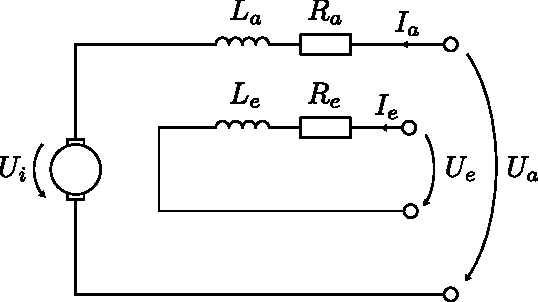
\includegraphics[scale=\schscale]{dc-motor.pdf}
\caption{Ersatzschaltbild einer DC-Maschine}
\label{sch:dc-maschine}
\end{figure}

\subsection{Verhalten und Kennlinie}

Eine DC- oder Gleichstrommaschine hat grundsätzlich drei Betriebszustände:
\begin{itemize}
	\item Ankerstellbereich
	\item Normbereich
	\item Feldschwächungsbereich
\end{itemize}

\begin{figure}[h!]
\centering
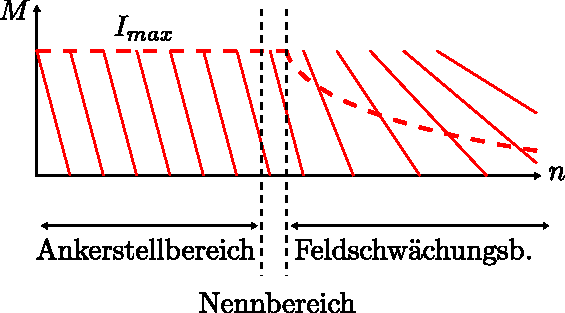
\includegraphics[scale=\schscale]{dc-motor-plot1.pdf}
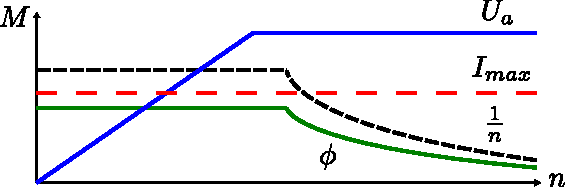
\includegraphics[scale=\schscale]{dc-motor-plot2.pdf}
\caption{Kennlinie einer DC-Maschine}
\label{fig:dc-motor-kennlinie}
\end{figure}

\noindent
Wichtig sind die foldengen Charakteristiken einer DC-Maschine:

\begin{itemize}
	\item Die Drehzahl ist proportional zur Spannung (falls unbelastet).
	\item Nimmt man der DC-Maschine Moment ab (d.h. belasten), so sinkt
		die Drehzahl linear ab bis hin zum maximalen Strom.
	\item	Blockiert man die Rotation (Reibung, Last) so überhitzt
		der Motor.
\end{itemize}

\subsection{Dynamischer Betrieb}
\[ \begin{array}{l}
U_a = U_i + (R_a \cdot I_a) + \left(L_a \cdot \frac{d I_a}{d t}\right) \\\\
U_e = (R_e \cdot I_e) + \left(L_e \cdot \frac{d I_e}{d t}\right) \\\\
U_i = c \cdot \Phi \cdot \omega_m \\\\
M_{el} = c \cdot \Phi \cdot I_a \\\\
M_{el} = M_{Welle} + M_{Reibung} + \left( J \cdot \frac{d \omega_m}{d t} \right) \\\\
\Phi = \frac{L_e}{N_e} \cdot I_e
\end{array} \]

\subsection{Stationärer Betrieb}
\[ \begin{array}{l}
U_a = U_i + (R_a \cdot I_a) \\\\
U_a = (c \cdot \phi \cdot \omega_m) + (R_a \cdot I_a) \\\\
\omega_m 
	= \frac{U_a - (R_a \cdot I_a)}{c \cdot \phi}
	= \frac{U_a}{c \cdot \phi} - \frac{R_a}{c \cdot \phi} \cdot I_a
	= \frac{U_a}{c \cdot \phi} - \frac{R_a}{(c \cdot \phi)^2} \cdot M
\end{array} \]




% coding:utf-8

%FOSAET, a LaTeX-Code for a electrical summary of basic electronics
%Copyright (C) 2013, Daniel Winz, Ervin Mazlagic

%This program is free software; you can redistribute it and/or
%modify it under the terms of the GNU General Public License
%as published by the Free Software Foundation; either version 2
%of the License, or (at your option) any later version.

%This program is distributed in the hope that it will be useful,
%but WITHOUT ANY WARRANTY; without even the implied warranty of
%MERCHANTABILITY or FITNESS FOR A PARTICULAR PURPOSE.  See the
%GNU General Public License for more details.
%----------------------------------------

\chapter{Digitaltechnik}
\newpage
% coding:utf-8

%FOSAET, a LaTeX-Code for a electrical summary of basic electronics
%Copyright (C) 2013, Daniel Winz, Ervin Mazlagic

%This program is free software; you can redistribute it and/or
%modify it under the terms of the GNU General Public License
%as published by the Free Software Foundation; either version 2
%of the License, or (at your option) any later version.

%This program is distributed in the hope that it will be useful,
%but WITHOUT ANY WARRANTY; without even the implied warranty of
%MERCHANTABILITY or FITNESS FOR A PARTICULAR PURPOSE.  See the
%GNU General Public License for more details.
%----------------------------------------

\section{Logische Verknüpfungen}

\subsection{NOT}
\begin{figure}[h!]
  \begin{subfigure}{0.3\textwidth}
    \[ X = \overline{A} \]
    \begin{tikztimingtable}
      A & lHLh \\
      X & hLHl \\
    \end{tikztimingtable}
  \end{subfigure}
  \begin{subfigure}{0.15\textwidth}
    \begin{tikzpicture}[circuit logic IEC]
      \node [not gate] (g) {};
      \draw (g.input) -- ++(left:3mm);
      \draw (g.output) -- ++(right:3mm);
    \end{tikzpicture}
  \end{subfigure}
  \begin{subfigure}{0.3\textwidth}
    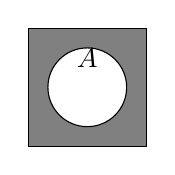
\begin{tikzpicture}[scale=0.5]
      \fill[gray] (-1.5,-1.5) rectangle (1.5,1.5);
      \draw (-1.5,-1.5) rectangle (1.5,1.5);
      \fill[white] (0,0) circle (1cm);
      \draw (0,0) circle (1cm);
      \draw (0,0.75) node {$A$};
    \end{tikzpicture}
  \end{subfigure}
  \begin{subfigure}{0.2\textwidth}
    \[ \begin{array}{c|c}
    A&X\\
    \hline
    0&1\\
    1&0
    \end{array} \]
  \end{subfigure}
\end{figure}

\subsection{OR}
\begin{figure}[h!]
  \begin{subfigure}{0.3\textwidth}
    \[ X = A \lor B \]
    \begin{tikztimingtable}
      A & lLHLHl \\
      B & lLLHHl \\
      X & lLHHHl \\
    \end{tikztimingtable}
  \end{subfigure}
  \begin{subfigure}{0.15\textwidth}
    \begin{tikzpicture}[circuit logic IEC]
      \node [or gate] (g) {};
      \draw (g.input 1) -- ++(left:3mm);
      \draw (g.input 2) -- ++(left:3mm);
      \draw (g.output) -- ++(right:3mm);
    \end{tikzpicture}
  \end{subfigure}
  \begin{subfigure}{0.3\textwidth}
    \begin{venndiagram2sets}[tikzoptions={scale=0.5}]
      \fillA \fillB
    \end{venndiagram2sets}
  \end{subfigure}
  \begin{subfigure}{0.2\textwidth}
    \[ \begin{array}{cc|c}
    A&B&X\\
    \hline
    0&0&0\\
    0&1&1\\
    1&0&1\\
    1&1&1
    \end{array} \]
  \end{subfigure}
\end{figure}

\subsection{NOR}
\begin{figure}[h!]
  \begin{subfigure}{0.3\textwidth}
    \[ X = \overline{A \lor B} \]
    \begin{tikztimingtable}
      A & lLHLHl \\
      B & lLLHHl \\
      X & hHLLLh \\
    \end{tikztimingtable}
  \end{subfigure}
  \begin{subfigure}{0.15\textwidth}
    \begin{tikzpicture}[circuit logic IEC]
      \node [nor gate] (g) {};
      \draw (g.input 1) -- ++(left:3mm);
      \draw (g.input 2) -- ++(left:3mm);
      \draw (g.output) -- ++(right:3mm);
    \end{tikzpicture}
  \end{subfigure}
  \begin{subfigure}{0.3\textwidth}
    \begin{venndiagram2sets}[tikzoptions={scale=0.5}]
      \fillNotAorB
    \end{venndiagram2sets}
  \end{subfigure}
  \begin{subfigure}{0.2\textwidth}
    \[ \begin{array}{cc|c}
    A&B&X\\
    \hline
    0&0&1\\
    0&1&0\\
    1&0&0\\
    1&1&0
    \end{array} \]
  \end{subfigure}
\end{figure}

\subsection{AND}
\begin{figure}[h!]
  \begin{subfigure}{0.3\textwidth}
    \[ X = A \land B \]
    \begin{tikztimingtable}
      A & lLHLHl \\
      B & lLLHHl \\
      X & lLLLHl \\
    \end{tikztimingtable}
  \end{subfigure}
  \begin{subfigure}{0.15\textwidth}
    \begin{tikzpicture}[circuit logic IEC]
      \node [and gate] (g) {};
      \draw (g.input 1) -- ++(left:3mm);
      \draw (g.input 2) -- ++(left:3mm);
      \draw (g.output) -- ++(right:3mm);
    \end{tikzpicture}
  \end{subfigure}
  \begin{subfigure}{0.3\textwidth}
    \begin{venndiagram2sets}[tikzoptions={scale=0.5}]
      \fillACapB
    \end{venndiagram2sets}
  \end{subfigure}
  \begin{subfigure}{0.2\textwidth}
    \[ \begin{array}{cc|c}
    A&B&X\\
    \hline
    0&0&0\\
    0&1&0\\
    1&0&0\\
    1&1&1
    \end{array} \]
  \end{subfigure}
\end{figure}

\newpage

\subsection{NAND}
\begin{figure}[h!]
  \begin{subfigure}{0.3\textwidth}
    \[ X = \overline{A \land B} \]
    \begin{tikztimingtable}
      A & lLHLHl \\
      B & lLLHHl \\
      X & hHHHLh \\
    \end{tikztimingtable}
  \end{subfigure}
  \begin{subfigure}{0.15\textwidth}
    \begin{tikzpicture}[circuit logic IEC]
      \node [nand gate] (g) {};
      \draw (g.input 1) -- ++(left:3mm);
      \draw (g.input 2) -- ++(left:3mm);
      \draw (g.output) -- ++(right:3mm);
    \end{tikzpicture}
  \end{subfigure}
  \begin{subfigure}{0.3\textwidth}
    \begin{venndiagram2sets}[tikzoptions={scale=0.5}]
      \fillNotAorNotB
    \end{venndiagram2sets}
  \end{subfigure}
  \begin{subfigure}{0.2\textwidth}
    \[ \begin{array}{cc|c}
    A&B&X\\
    \hline
    0&0&1\\
    0&1&1\\
    1&0&1\\
    1&1&0
    \end{array} \]
  \end{subfigure}
\end{figure}

\subsection{XOR}
\begin{figure}[h!]
  \begin{subfigure}{0.3\textwidth}
    \[ X = A \oplus B \]
    \begin{tikztimingtable}
      A & lLHLHl \\
      B & lLLHHl \\
      X & lLHHLl \\
    \end{tikztimingtable}
  \end{subfigure}
  \begin{subfigure}{0.15\textwidth}
    \begin{tikzpicture}[circuit logic IEC]
      \node [xor gate] (g) {};
      \draw (g.input 1) -- ++(left:3mm);
      \draw (g.input 2) -- ++(left:3mm);
      \draw (g.output) -- ++(right:3mm);
    \end{tikzpicture}
  \end{subfigure}
  \begin{subfigure}{0.3\textwidth}
    \begin{venndiagram2sets}[tikzoptions={scale=0.5}]
      \fillANotB \fillBNotA
    \end{venndiagram2sets}
  \end{subfigure}
  \begin{subfigure}{0.2\textwidth}
    \[ \begin{array}{cc|c}
    A&B&X\\
    \hline
    0&0&0\\
    0&1&1\\
    1&0&1\\
    1&1&0
    \end{array} \]
  \end{subfigure}
\end{figure}

\subsection{XNOR}
\begin{figure}[h!]
  \begin{subfigure}{0.3\textwidth}
    \[ X = \overline{A \oplus B} \]
    \begin{tikztimingtable}
      A & lLHLHl \\
      B & lLLHHl \\
      X & hHLLHh \\
    \end{tikztimingtable}
  \end{subfigure}
  \begin{subfigure}{0.15\textwidth}
    \begin{tikzpicture}[circuit logic IEC]
      \node [xnor gate] (g) {};
      \draw (g.input 1) -- ++(left:3mm);
      \draw (g.input 2) -- ++(left:3mm);
      \draw (g.output) -- ++(right:3mm);
    \end{tikzpicture}
  \end{subfigure}
  \begin{subfigure}{0.3\textwidth}
    \begin{venndiagram2sets}[tikzoptions={scale=0.5}]
      \fillNotAorB \fillACapB
    \end{venndiagram2sets}
  \end{subfigure}
  \begin{subfigure}{0.2\textwidth}
    \[ \begin{array}{cc|c}
    A&B&X\\
    \hline
    0&0&1\\
    0&1&0\\
    1&0&0\\
    1&1&1
    \end{array} \]
  \end{subfigure}
\end{figure}

% coding:utf-8

%FOSAET, a LaTeX-Code for a electrical summary of basic electronics
%Copyright (C) 2013, Daniel Winz, Ervin Mazlagic

%This program is free software; you can redistribute it and/or
%modify it under the terms of the GNU General Public License
%as published by the Free Software Foundation; either version 2
%of the License, or (at your option) any later version.

%This program is distributed in the hope that it will be useful,
%but WITHOUT ANY WARRANTY; without even the implied warranty of
%MERCHANTABILITY or FITNESS FOR A PARTICULAR PURPOSE.  See the
%GNU General Public License for more details.
%----------------------------------------
\section{Schreibweise logischer Funktionen}
\[ \text{ NOT }y = \neg y = \overline{y} \]
\[ x\text{ OR }y = x \lor y = x + y \]
\[ x\text{ AND }y = x \land y = x \cdot y \]
\[ x\text{ XOR }y = x \underline{\lor} y = x \oplus y \]

\section{Boolesche Algebra}
\[ \begin{array}{lllll} \overline{\overline{x}} = x &
x \land x = x & 
x \land \overline{x} = 0 &
x \lor x = x &
x \lor \overline{x} = 1 \end{array} \]
\[ \begin{array}{llll} x \land 0 = 0 & 
x \land 1 = x & 
x \lor 0 = x & 
x \lor 1 = 1 \end{array}\]
\[ \begin{array}{ll}
x \land y = y \land x & 
x \lor y = y \lor x \\\\ 
\overline{x} \land \overline{y} = \overline{x \lor y} & 
\overline{x} \lor \overline{y} = \overline{x \land y} \\\\ 
\overline{\overline{x} \land \overline{y}} = x \lor y & 
\overline{\overline{x} \lor \overline{y}} = x \land y \\\\ 
x \land (x \lor y) = x & x \lor (x \land y) = x \\\\ 
x \land (\overline{x} \lor y) = x \land y & 
x \lor (\overline{x} \land y) = x \lor y \\\\ 
(x \land y) \lor (\overline{x} \land y = y) & 
(x \lor y) \land (\overline{x} \lor y = y) \\ 
\end{array} \]
\[  \]

\input{kvmacros}

\section{Test für KV-Map}

\begin{figure}[h!]
\begin{minipage}{0.35\textwidth}
	\begin{tabular}{cccc|c}
		a
		& b
		& c
		& d
		&$y$\\
		\hline
		0 & 0 & 0 & 0 & 1 \\
		0 & 0 & 0 & 1 & 0 \\
		0 & 0 & 1 & 0 & 0 \\
		0 & 0 & 1 & 1 & 1 \\
		%\hline
		0 & 1 & 0 & 0 & 1 \\
		0 & 1 & 0 & 1 & 0 \\
		0 & 1 & 1 & 0 & 0 \\
		0 & 1 & 1 & 1 & 1 \\
		%\hline
		1 & 0 & 0 & 0 & 1 \\
		1 & 0 & 0 & 1 & 0 \\
		1 & 0 & 1 & 0 & 0 \\
		1 & 0 & 1 & 1 & 1 \\
		%\hline
		1 & 1 & 0 & 0 & 1 \\
		1 & 1 & 0 & 1 & 0 \\
		1 & 1 & 1 & 0 & 0 \\
		1 & 1 & 1 & 1 & 1 \\
		%\hline
	\end{tabular}
	%\caption{Wahrheitstabelle zu~\ref{kvmap_a}}
	%\label{truthtable_a}
\end{minipage}
\begin{minipage}{0.1\textwidth}
	\Huge$\Rightarrow$\normalsize
\end{minipage}
\begin{minipage}{0.5\textwidth}
	\kvnoindex
	\karnaughmap{4}
	            {$y$}
		    {dcba}
		    {1001100110011001}
		    {}
	\karnaughmap{4}
	            {$y$}
		    {dcba}
		    {1001100110011001}
		    {%
			\thicklines
% 			\textcolor{red}{
% 			\put(2,2){\oval(1.9,1.9)}
% 			\textcolor{blue}{
% 			\put(0,0){\oval(1.9,1.9)[rt]}
% 			\put(0,4){\oval(1.9,1.9)[rb]}
% 			\put(4,0){\oval(1.9,1.9)[lt]}
% 			\put(4,4){\oval(1.9,1.9)[lb]}}}}
}\end{minipage}
\end{figure}
\begin{lstlisting}[caption=Karnaugh-Diagramm]{karnaugh1}
% Karnaugh-Diagramm : 

\karnaughmap{4}
            {$y$}
            {dcba}
            {1001100110011001}
            {}
\end{lstlisting}

\begin{lstlisting}[caption=Karnaugh-Diagramm mit Vereinfachungen]{karnaugh2}
% Karnaugh-Diagramm mit Vereinfachungen

\karnaughmap{4}
            {$y$}
            {dcba}
            {1001100110011001}
            {\thicklines
             \textcolor{red}{
             \put(2,2){\oval(1.9,1.9)}
             \textcolor{blue}{
             \put(0,0){\oval(1.9,1.9)[rt]}
             \put(0,4){\oval(1.9,1.9)[rb]}
             \put(4,0){\oval(1.9,1.9)[lt]}
             \put(4,4){\oval(1.9,1.9)[lb]}}}}
\end{lstlisting}

% coding:utf-8

%FOSAET, a LaTeX-Code for a electrical summary of basic electronics
%Copyright (C) 2013, Daniel Winz, Ervin Mazlagic

%This program is free software; you can redistribute it and/or
%modify it under the terms of the GNU General Public License
%as published by the Free Software Foundation; either version 2
%of the License, or (at your option) any later version.

%This program is distributed in the hope that it will be useful,
%but WITHOUT ANY WARRANTY; without even the implied warranty of
%MERCHANTABILITY or FITNESS FOR A PARTICULAR PURPOSE.  See the
%GNU General Public License for more details.
%----------------------------------------

\section{Formelsammlung}
% \begin{figure}[h!]
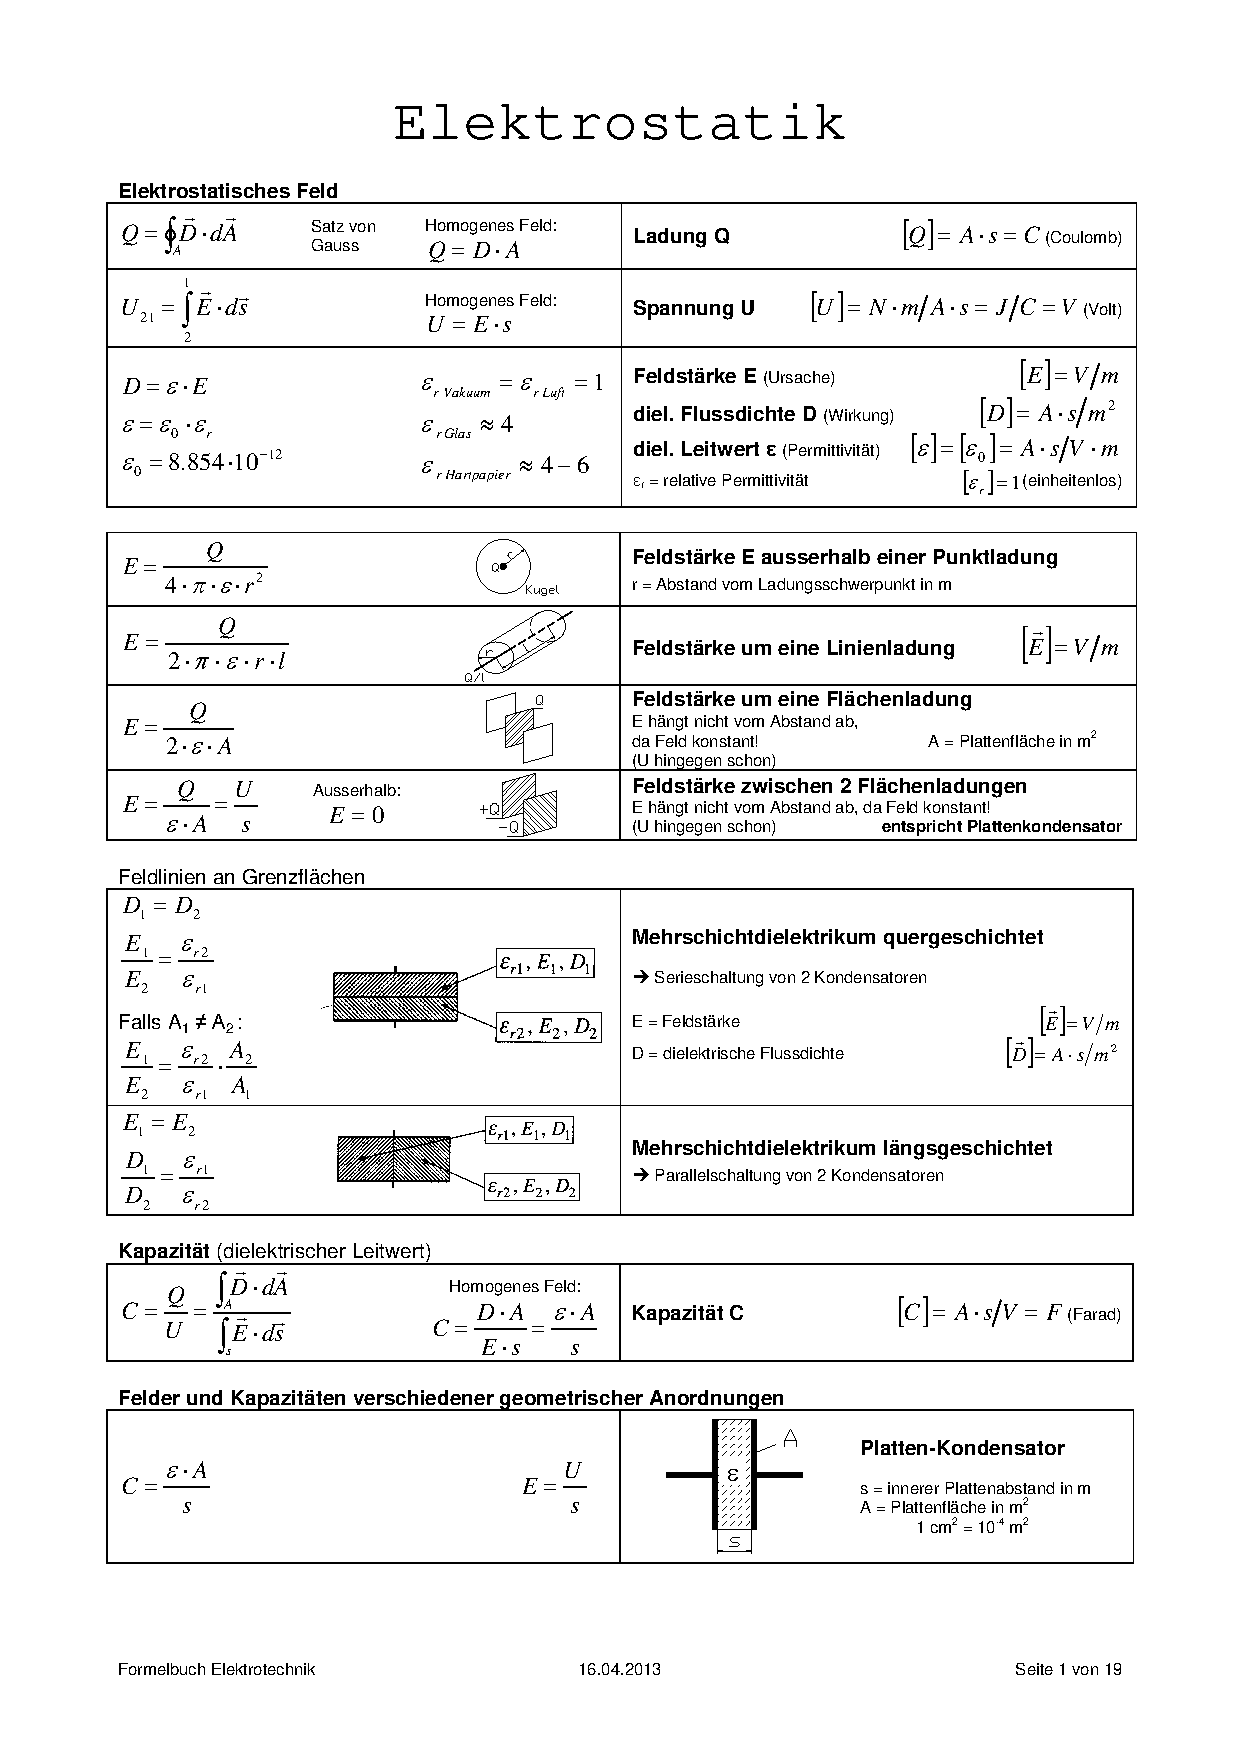
\includegraphics[page=1,scale=0.57,trim=20mm 20mm 20mm 20mm]{ET-Formelsammlung}
% \end{figure}
\newpage
% \begin{figure}[h!]
\includegraphics[page=2,scale=0.57,trim=20mm 20mm 20mm 20mm]{ET-Formelsammlung}
% \end{figure}
\newpage
% \begin{figure}[h!]
\includegraphics[page=3,scale=0.57,trim=20mm 20mm 20mm 20mm]{ET-Formelsammlung}
% \end{figure}
\newpage
% \begin{figure}[h!]
\includegraphics[page=4,scale=0.57,trim=20mm 20mm 20mm 20mm]{ET-Formelsammlung}
% \end{figure}
\newpage
% \begin{figure}[h!]
\includegraphics[page=5,scale=0.57,trim=20mm 20mm 20mm 20mm]{ET-Formelsammlung}
% \end{figure}
\newpage
% \begin{figure}[h!]
\includegraphics[page=6,scale=0.57,trim=20mm 20mm 20mm 20mm]{ET-Formelsammlung}
% \end{figure}
\newpage
% \begin{figure}[h!]
\includegraphics[page=7,scale=0.57,trim=20mm 20mm 20mm 20mm]{ET-Formelsammlung}
% \end{figure}
\newpage
% \begin{figure}[h!]
\includegraphics[page=8,scale=0.57,trim=20mm 20mm 20mm 20mm]{ET-Formelsammlung}
% \end{figure}
\newpage
% \begin{figure}[h!]
\includegraphics[page=9,scale=0.57,trim=20mm 20mm 20mm 20mm]{ET-Formelsammlung}
% \end{figure}
\newpage
% \begin{figure}[h!]
\includegraphics[page=10,scale=0.57,trim=20mm 20mm 20mm 20mm]{ET-Formelsammlung}
% \end{figure}
\newpage
% \begin{figure}[h!]
\includegraphics[page=11,scale=0.57,trim=20mm 20mm 20mm 20mm]{ET-Formelsammlung}
% \end{figure}
\newpage
% \begin{figure}[h!]
\includegraphics[page=12,scale=0.57,trim=20mm 20mm 20mm 20mm]{ET-Formelsammlung}
% \end{figure}
\newpage
% \begin{figure}[h!]
\includegraphics[page=13,scale=0.57,trim=20mm 20mm 20mm 20mm]{ET-Formelsammlung}
% \end{figure}
\newpage
% \begin{figure}[h!]
\includegraphics[page=14,scale=0.57,trim=20mm 20mm 20mm 20mm]{ET-Formelsammlung}
% \end{figure}
\newpage
% \begin{figure}[h!]
\includegraphics[page=15,scale=0.57,trim=20mm 20mm 20mm 20mm]{ET-Formelsammlung}
% \end{figure}
\newpage
% \begin{figure}[h!]
\includegraphics[page=16,scale=0.57,trim=20mm 20mm 20mm 20mm]{ET-Formelsammlung}
% \end{figure}
\newpage
% \begin{figure}[h!]
\includegraphics[page=17,scale=0.57,trim=20mm 20mm 20mm 20mm]{ET-Formelsammlung}
% \end{figure}
\newpage
% \begin{figure}[h!]
\includegraphics[page=18,scale=0.57,trim=20mm 20mm 20mm 20mm]{ET-Formelsammlung}
% \end{figure}
\newpage
% \begin{figure}[h!]
\includegraphics[page=19,scale=0.57,trim=20mm 20mm 20mm 20mm]{ET-Formelsammlung}
% \end{figure}
\\
\\
Quelle: Ilias ET2

\end{document}

